%----------------------------------------------------------------------------------------------
% Template padrão MACRO:
%
%	MANUAL DO DESENVOLVEDOR
%
%----------------------------------------------------------------------------------------------

% configura o documento:
\documentclass[12pt,a4paper,twoside,brazil,portugues,english]{book}

% pacotes mínimos:
\usepackage[utf8]{inputenc}
\usepackage[T1]{fontenc}

\usepackage[brazil]{babel}
\usepackage[a4paper,top=30mm,bottom=30mm,inner=30mm,outer=25mm,headheight=7mm,headsep=6mm,footskip=7mm]{geometry}

\usepackage{graphicx}
\usepackage{fancyhdr}
\pagestyle{fancy}

\PassOptionsToPackage{hyphens}{url}\usepackage[colorlinks]{hyperref}

% parâmetros pro template:
\newcommand{\surname}{Lara}
\newcommand{\initials}{AVL}
\newcommand{\reportnumber}{1}
\newcommand{\reportversion}{.00}
\newcommand{\reporttitle}{Manual do Desenvolvedor}
\newcommand{\registrationnumber}{ }
\newcommand{\studentname}{Arthur Viana Lara}
\newcommand{\advisorname}{Guilherme Vianna Raffo}
%\newcommand{\coadvisorname}{Brenner Reggo Santana}
\newcommand{\assunto}{Manual de utilização do simulador ProVant para o desenvolvedor.}
\makeatletter

% pacotes extras:
\usepackage{algorithmic}
\usepackage{color}
\usepackage{xcolor}

\hypersetup{
	pdftitle={\reporttitle}, 
	pdfauthor={\studentname},
    	pdfsubject={\assunto},
	pdfcreator={LaTeX with abnTeX2},
	pdfkeywords={abnt}{latex}{abntex}{abntex2}{trabalho acadêmico}, 
	colorlinks=true,  
	linkcolor=blue, 
	citecolor=blue,   
	filecolor=magenta,
	urlcolor=blue,
	bookmarksdepth=4
}

\usepackage{float}
\usepackage{enumitem}
\usepackage[newfloat]{minted}
\usepackage{caption}

\newenvironment{code}{\captionsetup{type=listing}}{}
\SetupFloatingEnvironment{listing}{name=Código}

\definecolor{LightGray}{gray}{0.9}
\definecolor{DarkGray}{gray}{0.1}

%\pagecolor{DarkGray}

%New colors defined below
\definecolor{codegreen}{rgb}{0,0.6,0}
\definecolor{codegray}{rgb}{0.5,0.5,0.5}
\definecolor{codepurple}{rgb}{0.58,0,0.82}
\definecolor{backcolour}{rgb}{0.95,0.95,0.92}



\makeatother

\usepackage{bookmark}
\bookmarksetup{
  open,
  numbered,
}

% configura a arvore de diretórios:
\usepackage[edges]{forest}

\definecolor{foldercolor}{RGB}{124,166,198}

\tikzset{pics/folder/.style={code={%
    \node[inner sep=0pt, minimum size=#1](-foldericon){};
    \node[folder style, inner sep=0pt, minimum width=0.3*#1, minimum height=0.6*#1, above right, xshift=0.05*#1] at (-foldericon.west){};
    \node[folder style, inner sep=0pt, minimum size=#1] at (-foldericon.center){};}
    },
    pics/folder/.default={20pt},
    folder style/.style={draw=foldercolor!80!black,top color=foldercolor!40,bottom color=foldercolor}
}

\forestset{is file/.style={edge path'/.expanded={%
        ([xshift=\forestregister{folder indent}]!u.parent anchor) |- (.child anchor)},
        inner sep=1pt},
    this folder size/.style={edge path'/.expanded={%
        ([xshift=\forestregister{folder indent}]!u.parent anchor) |- (.child anchor) pic[solid]{folder=#1}}, inner xsep=0.6*#1},
    folder tree indent/.style={before computing xy={l=#1}},
    folder icons/.style={folder, this folder size=#1, folder tree indent=3*#1},
    folder icons/.default={12pt},
}

\makeindex
\def\baselinestretch{1.0}

%% craindo caixa de apresentação do terminal
\usepackage{tcolorbox}

\makeatletter
\tcbuselibrary{minted,skins}

\newtcblisting{bashcode}{
	listing engine=minted,
	colback=bashcodebg,
	colframe=black!70,
	listing only,
	minted style=bw,
	minted language=bash,
	minted options={texcl=true},
	left=1mm,
}
\definecolor{bashcodebg}{rgb}{0.85,0.85,0.85}
\makeatother
%%%%%%%%%%%%%%5



\bibliographystyle{apalike2}

\begin{document}
\selectlanguage{brazil}

% capa:
\newcommand{\macroheader}[4]{MACRO/#1--\the\year /#2/#3+Version-#4}


\lfoot{\noindent \macroheader{\surname}{\initials}{\reportnumber}{\reportversion}}


\cfoot{}


\rhead{\noindent 
\includegraphics[width=0.15\textwidth]{report_template/macro_inline}}


\rfoot{\thepage}


\lhead{\leftmark}

\thispagestyle{empty}

\noindent \begin{center}
\textbf{}%
\begin{minipage}[t]{1\columnwidth}%
\noindent \begin{center}
\textbf{}%
\begin{minipage}[c]{0.3\columnwidth}%
\noindent \begin{flushleft}

\includegraphics[width=1\textwidth]{report_template/macro_inline_name}
\par\end{flushleft}%
\end{minipage}\textbf{}%
\begin{minipage}[b]{0.7\textwidth}%
\noindent \begin{flushright}
\textbf{\macroheader{\surname}{\initials}{\reportnumber}{\reportversion}}
\par\end{flushright}%
\end{minipage}
\par\end{center}%
\end{minipage}
\par\end{center}

\noindent \rule[0.5ex]{1\textwidth}{1pt}

\bigskip{}


\begin{center}
\textbf{\Large{}Universidade Federal de Minas Gerais - UFMG}
\par\end{center}{\Large \par}

\begin{center}
\textbf{\large{}}
\par\end{center}{\large \par}

\vspace{6cm}


\begin{center}
{\LARGE{}\reporttitle}
\par\end{center}{\LARGE \par}

\vfill{}


%\textit{\emph{\large{}Student registration number: \registrationnumber}}{\large \par}

\textit{\emph{\large{}Autor: \autor}}{\large \par}

%\textit{\emph{\large{}Advisor: \advisorname}}{\large \par}

\textit{\emph{\large{}Versão: \version}}{\large \par}

\vspace{1cm}


\begin{flushright}
\textit{\emph{\today}}
\par\end{flushright}

\pagebreak{}


\pagenumbering{roman}

%tabelade conteúdo:
\selectlanguage{brazil}
\tableofcontents
\clearpage

%lista de figuras:
\listoffigures
\addcontentsline{toc}{chapter}{Lista de Figuras}
\selectlanguage{brazil}
\clearpage

% conteúdo do manual:
\pagenumbering{arabic}
\setcounter{page}{1}
\chapter{Visão Geral}


Veículos aéreos não tripulados (VANTs) são aeronaves equipadas com sistemas embarcados, sensores e atuadores que permitem a realização de voos autônomos ou remotamente controlados. Eles são comumente classificados em dois grupos: veículos de asas rotativas, como helicópteros e quadrotores, e veículos de asas fixas, como aviões. 

Há diversas aplicações para VANTs, alguns exemplos são:

\begin{itemize}
	\itemsep0em
	\item Pulverização de culturas;
	\item Condução de rebanhos;
	\item Monitoramento de estradas;
	\item Inspeção da linhas de energia;
	\item Entrega de suprimentos em locais de difícil acesso.
\end{itemize}

Este trabalho está associado ao ProVANT\footnote{provant.paginas.ufsc.br}. O ProVANT consiste em uma parceria entre a Universidade Federal de Santa Catarina e a Universidade Federal de Minas Gerais, com o objetivo de realizar pesquisas e desenvolver novas tecnologias para aperfeiçoar o desempenho de VANTs. Neste contexto, atualmente, o ProVANT está focado no desenvolvimento de VANTs Tilt-rotor.  O Tilt-rotor está ilustrada na Figura \ref{vant.jpg} e é uma aeronave que possui configuração híbrida, portanto apresenta as principais vantagens das aeronaves de asa fixa e de asa rotativa, como por exemplo consumo reduzido de energia em voos de cruzeiro e decolagem e pouso na vertical. Ele pode operar tanto em ambientes fechados quanto abertos.

\begin{figure*}[!ht]
	\centering
	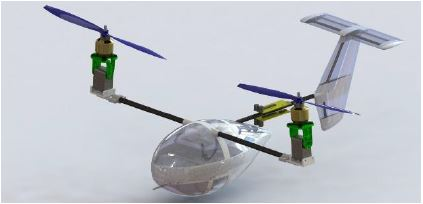
\includegraphics[width=0.8\textwidth]{figuras/VANT3.jpg}
	\caption{Tilt-rotor}
	\label{vant.jpg}
\end{figure*}

Com o intuito de fornecer uma ferramenta de testes para algoritmos e estratégias de controle voltados para vants, desenvolveu-se o simulador ProVANT. Pretende-se, dessa forma, reduzir de custos de projeto e tempo necessário para validação de novas tecnologias.

\section{Simuladores}

Simuladores voltados para aplicações de vants podem ser encontrados de duas maneiras: simuladores de voo e simuladores robóticos.

Simuladores de voo são ambientes desenvolvidos na maioria das vezes para treinamento de pilotos e/ou para desenvolvimento de jogos de aviões e helicópteros. X-plane e FlightGear são os simuladores mais utilizados por cientistas e profissionais da indústria aeronáutica.

Os simuladores robóticos são ambientes de desenvolvimento de simulação de robôs. O simulador Gazebo e o simulador V-rep são dois exemplos que se destacam nesta classe. Os simuladores robóticos são utilizados para testes e validação de algoritmos de controle e planejamento de trajetória. Estes trabalham com modelos de dinâmica multi-corpo com base nos conceitos de elos e juntas. 

A seguir será feito uma revisão bibliográfica sobre aplicações de vants em: i) X-plane; ii) Flightgear; iii) Gazebo; iv) V-rep.


\subsection{X-plane}

O X-plane\footnote{www.x-plane.com} é um simulador de voo multiplataforma (Linux, MAC e Windows) com a credencial da FAA (Administração Federal de Aviação) que simula voos baseado nos efeitos das forças sobre as múltiplas seções de uma aeronave. O X-plane inclui mais de 30 exemplares de aeronaves disponíveis para simulação e possui a capacidade de customização de cenário e importação de novas aeronaves. Esse simulador permite ao usuário configurar diferentes superfícies de controle aerodinâmico e realizar comunicação externa via protocolo UDP. Além disso, realiza tratamento de diferentes condições atmosféricas de acordo com a altitude. No entanto, o simulador apresenta como desvantagens ser um software proprietário, incapaz de simular múltiplos objetos de simulação no mesmo computador e de realizar simulações com modelos multi-corpos.

Em \cite{Figueiredo2012} foi modelado e simulado um quadrotor no simulador X-plane. A modelagem baseou-se numa aeronave desenvolvida por um grupo de pesquisa do Instituto Tecnológico da Aeronáutica, sendo utilizado o Matlab/Simulink para realizar o controle automático do quadrotor. Em \cite{Castro2014} e \cite{Garcia2010}, desenvolveu-se um ambiente de simulação para múltiplos VANTs na configuração quadrotor de forma semelhante a \cite{Figueiredo2012}. No entanto, devido ao elevado esforço computacional exigido pelo simulador, fez-se necessário a utilização de diversos computadores para a aplicação. Já em \cite{Bittar2014}, realizou-se uma simulação \textit{Hardware-in-the-loop} no X-plane de um veículo de asas fixas. Neste trabalho, o comportamento mecânico e aerodinâmico do VANT na configuração avião foi simulado pelo X-plane e o respectivo controlador foi implementado por um sistema embarcado. A comunicação entre o simulador X-plane e o controlador foi realizada através de comunicação serial, sendo que o último recebe do simulador em tempo real os dados dos sensores e, após processamento do controlador, reenvia os sinais de controle.

\subsection{FlightGear}

O FlightGear\footnote{www.flightgear.org} é um software de simulação de voo multiplataforma de código aberto. É extensível e utiliza três modelos de dinâmica de voo: JSBSim,YASim e UIUC. 

JSBSim é um modelo de dinâmica de voo genérico com seis graus de liberdade, onde a aeronave é modelada utilizando um arquivo XML, em que se define as propriedades de massa, aerodinâmica e controle de voo. YASim é um modelo de dinâmica de voo que simula o efeito da corrente de ar nas diferentes partes da aeronave. Por fim, o UIUC é um modelo de dinâmica de voo que engloba em simulação um modelo de aerodinâmica não-linear. Ele resulta em simulações com maior grau de realismo, sobretudo em situações de atitudes extremas, como estol e elevado ângulo ataque.

O simulador possui um banco de modelos e cenários disponíveis (cerca de 20.000 aeroportos reais), é capaz de simular de forma precisa falhas de sistemas e instrumentos aeronáuticos. Porém, é incapaz de emular modelos multi-corpos e de realizar simulações com mais de um modelo concomitantemente.    

O FlightGear foi utilizado por \cite{Sorton2005} como simulador para VANTs na configuração avião, e como controlador foi utilizado Matlab/Simulink. Já em \cite{Butt01052016}, foi desenvolvido um algoritmo \textit{offline} de geração de trajetórias 4D (tempo, longitude, latitude e altitude) para um VANT de asas fixas, sendo utilizado o simulador FlightGear para validá-lo.

\subsection{Gazebo}

Gazebo\footnote{www.gazebosim.org} \'e um software livre de simula\c c\~ao rob\'otico desenvolvido pela OSRF (Open Source Robotics Foundation), capaz de simular eficientemente popula\c c\~oes de objetos em cen\'arios complexos, sejam eles ambientes externos ou internos.

Esse simulador é apropriado para simulações com múltiplos objetos e detecção de colisão, sendo estes constituídos de um ou mais corpos. Esse sistema possui um banco de sensores considerável (ao todo são 12, contendo a capacidade de criar sensores customizados) e permite ao usuário incluir novos cenários e objetos de simulação através de arquivos XML. Além disso, possibilita que o usuário realize simulações na nuvem, por exemplo em servidores da Amazon. 

Algumas simulações de VANTs utilizando o Gazebo são encontradas na literatura. Em \cite{Nagaty2013}, projetou-se um controlador em cascata utilizando a estratégia de controle não linear  \textit{Backstepping} para a malha de controle interna e um controlador PD na malha externa. Ademais, validou-se o controlador projetado utilizando ROS (Robotic Operating System) e Gazebo. Já em \cite{Martinez2013}, desenvolveu-se um sistema de visão 3D para helicópteros, o qual foi utilizado numa simulação com o Gazebo.

\subsection{V-REP}

V-rep\footnote{www.coppeliarobotics.com} \'e um software de simula\c c\~ao rob\'otico multi-plataforma, desenvolvido pela Coppelia Robotics, capaz de simular popula\c c\~oes de objetos multi-corpos. É um sistema com interface amigável e suporte a várias linguagens de programação, sendo capaz de tratar colisões entre objetos de simulação, criar novos cenários e importar novos modelos. 

Apesar de sua vasta utilização para sistemas robóticos, pouco se encontra sobre o uso do V-REP com VANTs. Em \cite{7158723}, apresentou-se um ambiente de simulação desenvolvido com V-REP e ROS. Esse cenário foi utilizado para sintonia de uma abordagem de controle para um VANT VTOL (acrônimo para  \textit{Vertical Take-Off and Landing}, que significa decolagem e aterrissagem vertical) baseada em visão computacional. Foi proposto um algoritmo de controle baseado em redes neurais, adotando um estimador de pose com base no conhecimento da posição do local de decolagem. 


\section{Requisitos de projeto software}

%\subsection{Requisitos de Projeto}
%\markright{\thesection ~~~ Objetivos}
%label{objetivos}

No inicio do projeto de desenvolvimento do simulador ProVANT, definiu-se os seguintes requisitos não funcionais:

\begin{itemize}
	\itemsep0em
	\item[i)] Funcionar sobre sistema operacional Ubuntu/Linux;
	\item[ii)] Ter licen\c ca de software livre;
	\item[iii)] Ser capaz de realizar tratamento de colis\~oes;
	\item[iv)] Emular modelos multi-corpos;
	\item[v)] Incluir modelos de simulação com projeto CAD (projetos realizados com auxílio de computadores).
\end{itemize}	


Quanto aos requisitos funcionais, definiu-se:

\begin{itemize}
	\itemsep0em
	\item[i)] Interface gráfica para configuração de elementos de simulação;
	\item[ii)] Conjunto de instrumentos para medição e controle de variáveis físicas; 
	\item[iii)] Controlador a ser configurado pelo usuário. 
\end{itemize} 

Tendo em vista os requisitos não funcionais do projeto, os simuladores de voo descritos não são adequados, pois estes não são capazes de trabalhar com modelos de simulação multi-corpos. Já os simuladores robóticos descritos atendem a quase todos esses requisitos. Ambos funcionam no sistema operacional Ubuntu/Linux, são capazes de emular modelos multi-corpos e fazem tratamento de colisões. 


Entre os simuladores robóticos, o Gazebo é único exemplar que apresenta licença de software livre e acesso externo aos parâmetros do modelo via arquivo XML, facilitando a criação, modificação e armazenamento de modelos de simulação. Porém a característica determinante para a escolha do simulador a ser utilizado foi a existência de suporte pelo Gazebo, no início deste trabalho (Setembro/2015), à atuação de juntas rotativas via conjugado mecânico, o que não ocorria no V-REP. Portanto, devido a essas características, o Gazebo foi o simulador selecionado como base de software de simulação.

\section{Softwares utilizados}

Além do software de simulação Gazebo, utilizou-se outros 2 componentes de software para o desenvolvimento do simulador ProVANT: a plataforma de desenvolvimento QT e o ROS (Robot Operating System). A seguir será dado uma visão geral de cada componente.

\subsubsection{QT}

Parte do ambiente de simulação ProVANT foi desenvolvido na linguagem C++, utilizando a IDE QtCreator e bibliotecas da plataforma QT versão 5. Qt é uma plataforma de desenvolvimento de aplicações multi-plataforma (hardware e software) com ou sem interface gráfica. O Qt é desenvolvido atualmente pela \textit{The Qt Company} e disponibiliza diversos recursos aos programadores, tais como acesso a banco de dados SQL, análise XML, análise JSON, gerenciamento de threads e suporte de rede.

\subsubsection{ROS}

Robot Operating System (ROS) é uma plataforma de desenvolvimento de código aberto baseado em Linux para desenvolvimento robótico. O ROS provê funcionalidades que vão desde abstração de hardware e controle em baixo nível de dispositivos até navegação, planejamento de movimento e simulação de alto nível. O sistema foi desenvolvido inicialmente em 2007 no Laboratório de Inteligência Artificial de Stanford e agora é mantido por Willow Garage, um centro de pesquisa em robótica e incubadora.

As aplicações ROS são organizadas em estruturas chamadas Stacks, que agregam os Pacotes (em inglês, Packages) onde se encontram os executáveis, códigos-fonte e bibliotecas. Cada um desses níveis contém um arquivo de manifesto (chamdo ''package.xml'') responsável pela descrição do conteúdo, facilitando o compartilhamento com a comunidade científica. 

O ROS é um sistema descentralizado que permite que aplicações sejam executadas de forma distribuída entre as máquinas. Quando um arquivo executável de um pacote é iniciado, este origina um ou mais nós. Os nós representam processos individuais que se comunicam através dos chamados tópicos. Essa estrutura abstrai um sistema de troca de mensagens assíncrono baseado em sockets. Os nós podem atuar como publicadores em múltiplos tópicos simultaneamente. Enquanto publicadores, um único tipo de dado pode ser postado em um certo tópico, normalmente à uma taxa constante.

O elemento final na estrutura do ROS é o chamado ROS Core (roscore), que é executado em uma única máquina e atua como o DNS (Domain Name System). Cada nó deve receber um identificador ROS Core (Uniform Resource Identifier - URI) para que, durante a execução, os nós possam notificar ao ROS Core que eles existem. Essa estratégia permite que os nós se comuniquem através de conexões remotas e locais online.

\section{Organização do manual}

O Texto está organizado como a seguir:

\begin{enumerate}
	\item Este capítulo introduz dá uma visão geral sobre o simulador ProVANT
	\item O segundo capítulo apresenta a estrutura do ambiente de simulação ProVANT;
	\item O terceiro capítulo organização do projeto de software, descrevendo a localização de arquivos e diretórios;
	\item O quarto capítulo descreve detalhes do projeto relativo ao simulador Gazebo. Será abordado sobre modelos, cenários e plugins;
	\item O quinto capítulo descreve detalhes do Controlador;
	\item O sexto capítulo descreve detalhes da Interface gráfica;
	\item O sétimo capítulo descreve como é o processo de inicialização de uma instância de simulação.
	\item O apêndice A descreve como se configurar um arquivo ''CMakeLists.txt'' genérico.
	\item O apêndice B descreve como se configurar um arquivo ''package.xml'' genérico.
\end{enumerate}





\chapter{Estrutura do simulador}

A estrutura geral do simulador é ilustrada na Figura \ref{Esquematico.jpg}. O ambiente de simulação é constituído de três componentes: i) simulador Gazebo; ii) Controlador; iii) Interface gráfica. 


\begin{figure}[H]
	\centering
	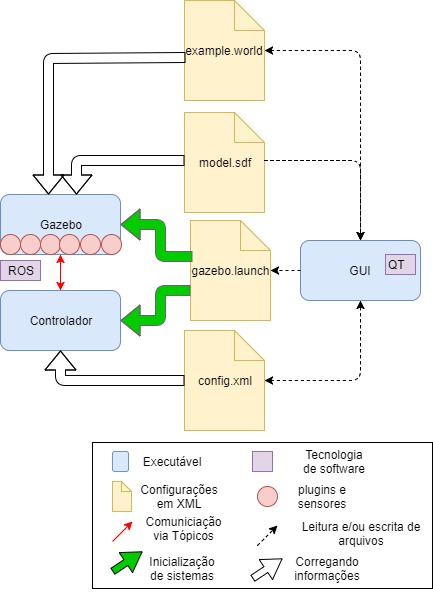
\includegraphics[width=0.65\textwidth]{figuras/estrutura.jpg}
	\caption{Esquemático do simulador}
	\label{Esquematico.jpg}
\end{figure}

O simulador Gazebo é o componente onde é executado o modelo do vant e, através de plugins e sensores, consegue-se obter e modificar dados durante execução do ambiente de simulação. Para sua configuração inicial, é necessário dois arquivos XML: ``model.sdf'' e ``example.world'' (pode-se escolher qualquer nome para este arquivo). Este descreve o cenário de simulação e aquele, o modelo de simulação.

O controlador, por sua vez, é o componente responsável por controlar o voo do vant. As configurações do controlador, tais como período de amostragem e tipo de estratégia de controle, são descritas em um arquivo denominado ``config.xml''.

Com o intuito de realizar comunicação entre Gazebo e Controlador e automatizar o seus respectivos processos de inicialização, utilizou-se características do ROS. A comunicação entre processos ocorre por meio de tópicos do ROS e a inicialização automática de processos, através de um arquivo XML denominado ``gazebo.launch''.

Por fim, com a finalidade de tornar amigável o processo de configuração da simulação, desenvolveu-se uma interface gráfica. A interface gráfica é um executável criado utilizando a API do QT, cuja função é ler e/ou editar os arquivos de configuração ``model.sdf'', ``gazebo.launch'' e ``config.xml'' (o sentido as setas na figura \ref{Esquematico.jpg} mostra o fluxo de informação entre o executável e tais arquivos).

Mais detalhes sobre tais elementos serão dados nos próximos capítulos do manual.


\chapter{Organização do projeto de software}

\hspace{1.5em}O diretório raíz do simulador é chamado \emph{ProVANT-Simulator}, no caso da versão estar no diretório destinado ao público, ou \emph{ProVANT-Simulator\_Developer}, para a versão em processo de desenvolvimento. Tal diretório está localizado, após a instalação, no diretório {\color{green}{\$HOME/catkin\_ws/src/}}. A figura \ref{fig:arvore_principal} ilustra a árvore de diretórios da estrutura do simulador ProVant. No diretório raíz, encontram-se duas pastas: \emph{doc} e \emph{source}: a pasta \emph{doc} contêm a documentação e os manuais de uso; e a pasta \emph{source} contêm o projeto de desenvolvimento da aplicação. 

\begin{figure}[htbp]
	\begin{forest}
		for tree={font=\sffamily, grow'=0,
			folder indent=.9em, folder icons,
			edge=densely dotted}
		[ProVANT-Simulator
		[ doc
		]
		[ source
		[build]
		[Database]
		[GUI]
		[Structure]
		]
		]
	\end{forest}
	\caption{Árvore dos diretórios principais do simulador ProVant.}
	\label{fig:arvore_principal}
\end{figure}

No primeiro nível da hierarquia do diretório raiz do simulador são encontrados os seguintes diretórios:

\begin{itemize}
	\itemsep0em
	\item \emph{build}: possui os arquivos binários  da interface gráfica. É gerado após a instalação completa do ambiente de simulação.
	\item \emph{Database}: possui arquivos de configuração de modelos, de cenários e da inicialização do ambiente de simulação.
	\item\emph{GUI}: possui o código fonte da interface gráfica.
	\item \emph{Structure}: possui o código fonte dos plugins e controlador; arquivos de dados gerados de simulação; e arquivos de descrição das mensagens de tópicos utilizadas para comunicação entre processos no ambiente de simulação. 
\end{itemize}



%\section{Diretório \emph{build}}
%\label{sec:d_build}
%
%\hspace{1.5em}O diretório \emph{build} contêm os arquivos binários, gerados pela compilação da interface gráfica.

\section{Diretório \emph{Database}}
\label{sec:d_database}

\hspace{1.5em}O diretório \emph{Database} é responsável por armazenar os cenários para o simulador, os modelos dos VANTs e arquivos de inicialização di ambiente de simulação. A estrutura interna do diretório  \emph{Database}, é ilustrado pela figura \ref{fig:arvore_database}.

\begin{tiny}
\begin{figure}[htbp]
\begin{forest}
	for tree={font=\sffamily, grow'=0,
    folder indent=.9em, folder icons,
    edge=densely dotted}
[Database
  [launch]
  [models]
  [worlds]
  [CMakeLists.txt, is file]
  [package.xml, is file]
]
\end{forest}
\caption{Árvore do diretório \emph{Database}.}
\label{fig:arvore_database}
\end{figure}
\end{tiny}

onde,

\begin{itemize}
	\itemsep0em
	\item \emph{launch}:  possui um arquivo denominado \emph{gazebo.launch}. Este é um arquivo escrito em \emph{XML} que se encarrega dos comandos de configuração do simulador, isto é, inicializa o ambiente do \emph{Gazebo} e executa o nó \emph{controller}.
	\item \emph{models}:  armazena modelos VANTs disponíveis.
	\item \emph{worlds}:  contem os arquivos de extensão \emph{world} correspondentes a descrição de cenários e configurações de simulação.
	\item \emph{CMakeLists.txt}: armazena informações para compilação de códigos fontes.
	\item \emph{package.xml}: armazena metadados do diretório, tais como nome e e enereço de e-mail do autor para contato. 
\end{itemize}

\section{Diretório \emph{GUI}}
\label{sec:d_GUI}

\hspace{1.5em}O diretório \emph{GUI} possui os arquivos \emph{.h} e \emph{.cpp} utilizados na implementação da interface gráfica.

\section{Diretório \emph{Structure}}
\label{sec:d_structure}

\hspace{1.5em}O diretório contém o código fonte de todos os componentes do ambiente de simulação, com exceção da interface gráfica. Além disso, é o local para armazenamento de arquivos de dados da simulação. A figura \ref{fig:arvore_structure} ilustra o diretório \emph{Structure}.

\begin{tiny}
\begin{figure}[H]
\begin{forest}
	for tree={font=\sffamily, grow'=0,
    folder indent=.9em, folder icons,
    edge=densely dotted}
  	[Structure
  		[Controller
  		]
  		[control\_strategies
  		]
  		[custom\_plugins
  		]
  		[Matlab
  		]
  		[simulator\_msgs
  		]
  	]
\end{forest}
\caption{Árvore do diretório \emph{Structure}.}
\label{fig:arvore_structure}
\end{figure}
\end{tiny}

\vspace{0.5em}
\noindent 

onde,

\begin{itemize}
	\itemsep0em
	\item \emph{Controller}: contem o código fonte do Controlador;
	\item \emph{control\_strategies}:contem o código fonte para diversas estratégias de controle;
	\item \emph{custom\_plugins}: possui o código fonte dos plugins.
	\item \emph{Matlab}: local onde se armazena arquivos com dados oriundos de simulações.
	\item \emph{simulator\_msgs}: contém arquivos de descrição de mensagens utilizadas para comunicação entre processos via tópicos do ROS. 
\end{itemize}

%\chapter{Simulador Gazebo}

%Este capítulo explicita três elementos do simulador Gazebo utilizados na criação do ambiente de desenvolvimento ProVANT: 
%
%\begin{itemize}
%	\item[\textbf{Modelo}] conjunto de arquivos com informações relativas à estrutura física do vant: características inerciais, visuais e de colisão.
%	\item[\textbf{Cenário}] arquivo de descrição de configurações da simulação, tal como passo de simulação, tipo de motor de simulação, elementos visuais (exemplo: ventos, céu, e cor do piso) e quantidade/pose inicial de modelos.
%	\item[\textbf{Plugin}] código fonte de criação de elementos sensoriais e de atuação do modelos.
%\end{itemize}

\chapter{Modelos}

\section{Organização e estrutura}


\begin{tiny}
	\begin{figure}[H]
		\begin{forest}
			for tree={font=\sffamily, grow'=0,
				folder indent=.9em, folder icons,
				edge=densely dotted}
			[vant\_x
			[config
			[config.xml, is file]  
			]
			[meshes
			[$\star$.stl,is file]
			]  
			[robot
			[model.sdf, is file]
			]
			[imagem.gif, is file]
			[model.config, is file]
			]
		\end{forest}
		\caption{Árvore ilustrativa para um diretório que descreve um VANT de versão x \emph{vant\_x}.}
		\label{fig:arvore_vantx}
	\end{figure}
\end{tiny}


Os arquivos associados aos modelos de VANTs, utilizados no ambiente de simulação ProVANT, estão localizados na pasta referênte ao caminho:

\begin{bashcode}
$HOME/catkin_ws/src/ProVANT-Simulator/source/Database/models/real
\end{bashcode}


Cada modelo no ambiente de simulação ProVant possui um diretório com o seu respectivo nome. Nesse diretório estão arquivos que descrevem os modelos dinâmicos, visuais, de colisão, sensoriais e da lei de controle utilizada. Portanto, caso seja necessário adicionar um novo modelo, ou editar um existente, o mesmo deve possuir arquivos de configuração/descrição do VANT organizados conforme ilustrado na Figura \ref{fig:arvore_vantx}. Os diretórios e arquivos necessários são:
 
\begin{itemize}
\item\emph{config}:  a pasta \emph{config} possui um único arquivo nomeado \emph{config.xml}. Este arquivo em \emph{XML} escreve configurações do Controlador, tais como período de amostragem e estratégia de controle a ser utilizada, e será explicitado no capítulo referente a descrição do elemento Controlador.
\item \emph{meshes}: a pasta contêm os arquivos de extensão \emph{.stl} que são obtidos no processo de importação do modelo em CAD do VANT pelo \emph{Solidworks}.
\item \emph{robot}: a pasta contêm um arquivo \emph{SDF} que descreve o VANT para o simulador.
\item \emph{imagem.gif}: corresponde à imagem do vant a ser utilizada na interface gráfica.
\item \emph{model.config}: arquivo \emph{XML} com informações sobre o modelo, o nome do desenvolvedor e as licenças de uso.
\end{itemize}



\section{Arquivo ''model.sdf''}


Antes de apresentar a configuração básica de um arquivo SDF, é necessário primeiro introduzir alguns conceitos. Um modelo corresponde a um sistema mecânico, que pode ser formado por um ou múltiplos corpos rígidos\footnote{Ao assumir um corpo como rígido são desprezando efeitos de elasticidade e deformações}. Assim como em um manipulador, no simulador os corpos são denominados elos. Elos filhos são conectados a elos pai através de juntas. Elos filhos são corpos rígidos que possuem movimento restringido pela conexão ("junta") com corpos denominados elos pai. Os elos possuem propriedades inerciais, visuais e de colisão. Já as juntas, impõem a restrição do movimento relativo entre dois elos, com propriedades como o tipo de junta (Prismática, rotativa, etc.), limites de movimento (Posição e velocidade), existência de atrito, etc. A Figura \ref{geral} ilustra um exemplo de arquivo SDF, onde:\small
\begin{itemize}
\setlength{\itemsep}{1pt}
\setlength{\parskip}{0pt}
\setlength{\parsep}{0pt}
\item[-] \textcolor{blue}{<link></link>}: especifica a existência de um elo, com o seu nome;
\item[-] \textcolor{blue}{<joint></joint>}: especifica a existência de uma junta, com o seu nome.  
\end{itemize}\normalsize

\begin{figure}[H]
\begin{minted}{xml}
<?xml version="1.0" encoding="UTF-8"?>
<sdf version="1.4">
	<model name="modelo">
		<link name="corpo">
		...
		</link>
		<link name="servo">
		...
		</link>
		<joint name="corpo_servo">
		...
		</joint>
	</model>
</sdf>
\end{minted}
\vspace{-1cm}
\caption{Descrição de um elo no arquivo ''modelo.sdf''}
\label{geral}
\end{figure}


Cada elo do modelo possui três tipos de descrições para o simulador: cinemática, visual e de colisão.  A estrutura de configuração de um elo em um arquivo SDF possui o formato ilustrado na Figura \ref{elo}, onde:
\small
\begin{itemize}
\setlength{\itemsep}{1pt}
\setlength{\parskip}{0pt}
\setlength{\parsep}{0pt}
\item[-] \textcolor{blue}{<pose></pose>}: define a pose do elo;
\item[-] \textcolor{blue}{<inertial></inertial>}: especifica as propriedades inerciais do elo;
\item[-] \textcolor{blue}{<collision></collision>}: especifica o modelo de colisão do elo. Os modelos de colisão dos VANTs usados no ambiente de simulação são obtidos de arquivos CAD;
\item[-] \textcolor{blue}{<visual></visual>}: especifica características visuais, como cor e formato. Os modelos visuais dos VANTs usados no ambiente de simulação são obtidos de arquivos CAD, exceto a cor, que é especificada separadamente.
\end{itemize}\normalsize

\begin{figure}[ht!]
\begin{minted}{xml}
<link name="servodir">
	<pose>0.02E-3 -277.61E-3 56.21E-3 -0.0872665 0 0</pose>
	<inertial> 
	...
	</inertial>
	<collision name="servodircollision"> <!--opcional-->
	...
	</collision>
	<visual name="servodirvisual"> <!--opcional-->
	...
	</visual>
</link>
\end{minted}
\vspace{-1cm}
\caption{Descrição da de um elo no ''modelo.sdf''}
\label{elo}
\end{figure}

\noindent \textbf{Parâmetros de inércia do elo}: O usuário deve informar os parâmetros de inércia de cada elo na \textit{tag} ''inertial''. As informações obrigatórias são a massa, posição relativa do centro de massa e o tensor de inércia. Na Figura \ref{inertial} é ilustrado um exemplo de configuração dos parâmetros de inércia de um elo em formato SDF, onde:
\small
\begin{itemize}
\setlength{\itemsep}{1pt}
\setlength{\parskip}{0pt}
\setlength{\parsep}{0pt}
\item[-] \textcolor{blue}{<mass></mass>}: define a massa do elo;
\item[-] \textcolor{blue}{<pose></pose>}: especifica a posição do centro de massa do elo em relação a seu sistema de coordenadas principal;
\item[-] \textcolor{blue}{<inertia></inertia>}: especifica o tensor de inércia do elo;
\end{itemize}\normalsize

\begin{figure}[H]
\begin{minted}{xml}
<inertial>
	<mass>0.0809439719362664</mass>
	<pose>
	-3.60859273452335E-10 -0.000226380714807978 0.0594780519701684 0 0 0
	</pose>
	<inertia>
		<ixx>3.88267747087835E-06</ixx>
		<ixy>6.03219085082653E-06</ixy>
		<ixz>-2.78471406661236E-12</ixz>
		<iyy>0.000104858690365283</iyy>
		<iyz>7.0486590219062E-07</iyz>
		<izz>8.31755564684115E-05</izz>		
	</inertia>
</inertial>
\end{minted}
\vspace{-0.8cm}
\caption{Descrição de características inerciais no arquivo ''modelo.sdf''}
\label{inertial}
\end{figure}


\noindent \textbf{Propriedades de colisão do elo}: Para que efeitos de colisão sejam aplicados ao elo, o usuário deve descrever o formato do elo no arquivo ''model.sdf''. Existem diversas formas de descrição, porém este manual apresenta apenas o método utilizado nos modelos de VANTs do ambiente de simulação ProVANT, que consiste na importação de arquivos criados através de ferramentas CAD, como o SolidWorks. A Figura \ref{colision} mostra um exemplo de descrição dos parâmetros visuais de um elo a partir de um arquivo STL, onde:
\small
\begin{itemize}
\setlength{\itemsep}{1pt}
\setlength{\parskip}{0pt}
\setlength{\parsep}{0pt}
\item[-] \textcolor{blue}{<pose></pose>}: especifica a pose do modelo colisão em relação ao centro de coordenadas do elo;
\item[-] \textcolor{blue}{<uri></uri>}: caminho do arquivo mesh, a partir do diretório do modelo, obtido via exportação no SolidWorks; 
\end{itemize} \normalsize

\begin{figure}[ht!]
\begin{minted}{xml}
<collision name="servodircollision">
	<pose>0 0 0 0 0 0</pose>
	<geometry>
		<mesh>
			<uri>model://vant_2comcarga/meshes/servodir.STL</uri>
		</mesh>
	</geometry>
</collision>
\end{minted}
\vspace{-0.8cm}
\caption{Descrição de características de colisão no arquivo ''model.sdf''}
\label{colision}
\end{figure}

\noindent \textbf{Propriedades visuais do elo}: Para que o elo seja visualizado durante a simulação, o usuário deve descrever os parâmetros visuais do elo no arquivo ''model.sdf''. Assim como no caso anterior, existem diversas formas de descrição, porém este manual ilustra apenas o método utilizado nos modelos de VANTs do ambiente de simulação, que consiste na importação de arquivos criados através de ferramentas CAD. A Figura \ref{visual} mostra um exemplo de descrição dos parâmetros visuais de um elo a partir de um arquivo STL, 	
onde: \small
\begin{itemize}
\setlength{\itemsep}{1pt}
\setlength{\parskip}{0pt}
\setlength{\parsep}{0pt}
\item[-] \textcolor{blue}{<pose></pose>}: especifica a pose que o modelo visual do elo será definido em relação ao sistema de coordenadas do elo;
\item[-] \textcolor{blue}{<uri></uri>}: caminho do arquivo mesh, a partir do diretório do modelo, obtido via exportação no SolidWorks;
\item[-] \textcolor{blue}{<ambient></ambient>}: definição de cor ambiente;
\item[-] \textcolor{blue}{<diffuse></diffuse>}: definição de cor difusa;
\item[-] \textcolor{blue}{<specular></specular>}: definição de cor especular;
\item[-] \textcolor{blue}{<emissive></emissive>}: definição de cor emissiva.
\end{itemize} \normalsize

\begin{figure}[ht!]
\begin{minted}{xml}
<visual name="servodirvisual">
	<pose>0 0 0 0 0 0</pose>
	<geometry>
		<mesh>
			<uri>model://vant_2comcarga/meshes/servodir.STL</uri>
		</mesh>
	</geometry>
	<material>
		<ambient>0 0 0 0</ambient>
		<diffuse>1 1 1 1</diffuse>
		<specular>0.1 0.1 0.1 1</specular>
		<emissive>0 0 0 0</emissive>
	</material>
</visual>
\end{minted}
\vspace{-0.8cm}
\caption{Descrição de características visuais no arquivo ''model.sdf''}
\label{visual}
\end{figure}

\subsubsection{Descrição de junta} 

Há 7 tipos de juntas no simulador: 

\begin{itemize}
\item \textbf{revolute}: junta rotativa; 
\item \textbf{gearbox}: junta rotativa com presença de engrenagens para transmissão de movimento angular entre elos com diferentes relações de torque e velocidade; 
\item \textbf{revolute2}: junta composta por duas juntas rotativas em série; 
\item \textbf{prismatic}: junta prismática; (\textbf{universal}), junta com comportamento de uma bola articulada; 
\item \textbf{piston}: junta com comportamento da combinação de uma junta rotativa e uma junta prismática.
\end{itemize}

Um exemplo de estrutura de configuração de uma junta é mostrado na Figura \ref{joint}, onde:
\begin{itemize}
\setlength{\itemsep}{1pt}
\setlength{\parskip}{0pt}
\setlength{\parsep}{0pt}
\item[-] \textcolor{blue}{<pose></pose>}: descreve a pose relativa em que o elo filho está em relação ao elo pai.
\item[-] \textcolor{blue}{<parent></parent>}: nome do elo pai.
\item[-] \textcolor{blue}{<child></child>}: nome do elo filho.
\item[-] \textcolor{blue}{<axis></axis>}: vetor unitário que corresponde ao eixo de rotação da junta. (expressado no sistema de coordenadas do modelo, se estiver utilizando a versão 1.4 do formato SDF; e expressado no sistema de coordenadas do elo filho, se estiver utilizando a versão 1.6 do formato SDF).
\item[-] \textcolor{blue}{<lower></lower>}: limite inferior de posição da junta (em rad, caso seja do tipo rotativa, e metros, caso seja prismática).
\item[-] \textcolor{blue}{<upper></upper>}: limite superior de posição da junta (em rad, caso seja do tipo rotativa, e metros, caso seja prismática).
\item[-] \textcolor{blue}{<velocity></velocity>}: limite de velocidade da junta (em rad/s, caso seja do tipo rotativa, e m/s, caso seja prismática).
\item[-] \textcolor{blue}{<effort></effort>}: limite de esforço da junta (em N.m, caso seja do tipo rotativa, e N, caso seja prismática).
\item[-] \textcolor{blue}{<damping></damping>}: coeficiente de atrito viscoso.
\item[-] \textcolor{blue}{<friction></friction>}: coeficiente de atrito estático.
\end{itemize}

\begin{figure}[ht!]
\begin{minted}{xml}
<joint name="aR" type="revolute">
	<pose>0 0 0 0 0 0</pose>
	<parent>corpo</parent>
	<child>servodir</child>
	<axis>
		<xyz>0 0.9962 -0.0872</xyz>
		<limit>
			<lower>-1.5</lower>
			<upper>1.5</upper>
			<effort>2</effort>
			<velocity>0.5</velocity>
		</limit>
		<dynamics>
			<damping>0</damping>
			<friction>0</friction>
		</dynamics>
	</axis>
</joint>
\end{minted}
\vspace{-0.8cm}
\caption{Descrição de juntas no arquivo ''model.sdf''}
\label{joint}
\end{figure}

\section{Arquivo ''model.config''}

No arquivo ''model.config'' o gazebo identifica onde está o arquivo com os dados estruturais do modelo, além de informações associadas à autoria, versão e descrição do modelo. A Figura \ref{model.config} ilustra um exemplo desse arquivo. As \textit{tags} utilizadas no arquivo ''model.config'' são:
\small
\begin{itemize}
\setlength{\itemsep}{1pt}
\setlength{\parskip}{0pt}
\setlength{\parsep}{0pt}
\item[-] \textcolor{blue}{<name></name>}: especifica o nome do modelo;
\item[-] \textcolor{blue}{<version></version>}: especifica a versão;
\item[-] \textcolor{blue}{<sdf></sdf>}: especifica o arquivo com a descrição do modelo dinâmico, de colisão e visual de modelo para o simulador Gazebo;
\item[-] \textcolor{blue}{<author><name></name></author>}\textcolor{blue}: especifica o nome do autor do modelo;
\item[-] \textcolor{blue}{<author><email></email></author>}: especifica o email para contato com o autor;
\item[-] \textcolor{blue}{<description></description>}: descreve brevemente o modelo.
\end{itemize}\normalsize

\begin{figure}[ht!]
\begin{minted}{xml}
<?xml version="1.0"?>
<model>
<name>vant</name>
<version>1.0</version>
<sdf version='1.5'>robot/model.sdf</sdf>
	<author>
	<name>provant</name>
	<email>provant@ufmg.br</email>
	</author>
		<description>
			The UAV version 3.0 of the provant project 
		</description>
	</model>
</sdf>
\end{minted}
\vspace{-0.8cm}
\caption{Exemplo de conteúdo existente no arquivo ''model.config''}
\label{model.config}
\end{figure}


\section{Arquivos ''meshes''}

''Mesh'' (do inglês, significa malha) é a representação de objetos virtuais/computacionais em várias áreas da tecnologia, sobretudo na resoluções de problemas de engenharia e é compostas por vértices, arestas e triângulos.

O simulador Gazebo consegue importar dois tipos de arquivos para representação de área e superfícies: arquivos STL e DAE, estes oriundos de softwares CAD. No ambiente de simulação ProVANT, cada modelo vant é formado por vários elos e cada elo terá respectivas representações visuais e de colisão. Por motivos de organização, definiu-se que e o diretório ''Meshes'' será o local para armazenamento de tais arquivos.

A seguir será demonstrado um passo a passo de como obter o modelo com seus respectivos arquivos de descrição visual e de colisão.    

\section{Obtenção de modelos a partir do SolidWorks}

Está subseção descreve o conjunto de passos necessários para a exportação de um projeto mecânico para o formato necessário para uso no simulador Gazebo. Atente-se à necessidade de realizar ajustes no desenho CAD para o processo de exportação tenha sucesso. 

\subsection{Ajustes no Desenho CAD }

Para poder exportar o modelo para o formato necessário para uso no simulador Gazebo é necessário realizar o \textit{download} e instalação do plugin ''Sw\_Urdf\_Exporter''. O plugin pode ser encontrado em \url{http://wiki.ros.org/sw_urdf_exporter}. 

Além de \textit{download} e instalação do plugin, é necessário garantir que não exista nenhuma peça com o valor da massa substituída manualmente. Isso gera inconsistências entre o modelo em CAD e o modelo exportado. Uma maneira solucionar este problema, é criar um material personalizado, com uma densidade que corresponda a massa desejada, tal valor é obtido através da relação entre massa e volume.

Outro ajuste importante é a definição de quantos elos deve ter o modelo. Neste manual, exemplifica-se o processo de exportação para o modelo VANT-3.0, ilustrado na Figura \ref{vant.jpg}.

O VANT 3.0, ao todo possui sete corpos:


\begin{description}
\item [main\_body] é o corpo referência do VANT-3.0, composto pelo Corpo, suporte dos motores e parte fixa da empenagem;
\item [motorR] é o grupo propulsor da direita com exceção da hélice; 
\item [motorL] é o grupo propulsor da esquerda com exceção da hélice; 
\item [propeller\_R] é a hélice da direita;
\item [propeller\_L] é a hélice da esquerda;
\item [elevator] é a parte móvel da empenagem horizontal;
\item [rudder] é a parte móvel da empenagem vertical.
\end{description}

É necessário criar um eixo de coordenadas no centro de massa de cada um dos corpos, para que possam ser referenciados no momento da exportação. No caso do VANT-3.0 são criados eixos de coordenadas sobre o eixo de rotação dos servos. Outro eixo além dos citados é a referência do main\_body, localizado onde, teoricamente, pode-se encotrar a IMU. É importante a criação de eixos, que determinam como os corpos se movimentam, já que só temos movimentos de revolução. No VANT-3.0 existem eixos criados no centro de rotação das hélices e nos servos.E também no profundor e no leme.

\subsection{Processo de Exportação}

O processo de exportação de um arquivo ''.sdlprt'' para ''.urdf'' é simples e intuitivo. O recurso se encontra em File->Export as URDF, o endereço pode mudar entre versões do SolidWorks®, no caso foi usada a de 2014.

\begin{figure}[!htb]% aqui começa o ambiente figura
\centering % este comando é para centralizar a figura
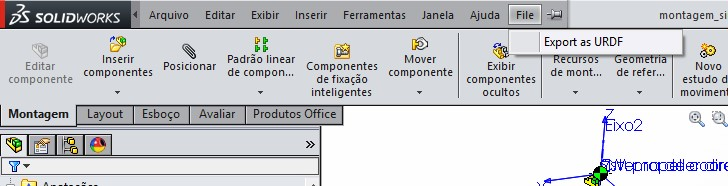
\includegraphics[scale=0.75]{Imagens/ExportasURDF.JPG} % aqui é onde chamamos a figura o que está entre [] são opções de formatação da figura e o que está entre {} é o nome da figura
\caption{Tela onde se inicia o processo} % esta é a legenda da figura
\end{figure} % aqui acaba o ambiente figura.


No canto direito da tela abrirá uma tela para inserir os parâmetros. Os primeiros parâmetros a inserir são sobre o link principal que serve de referência para o modelo, no caso do VANT-3.0 o main\_body. Os itens a serem detalhados estão listados abaixo:

\begin{description}
\item [Link Name] é o nome dado ao link principal do modelo a ser exportado;
\item [Global Origin Coordinate System] é o eixo de coordenadas que será a referência para esse link e para todo o modelo; 
\item [Link Components] local onde se define quais componentes do desenho CAD farão parte do link pai; 
\item [Number of child links] é onde se determina quantos links serão ligados ao link em questão;
\end{description}

\begin{figure}[!htb]% aqui começa o ambiente figura
\centering % este comando é para centralizar a figura
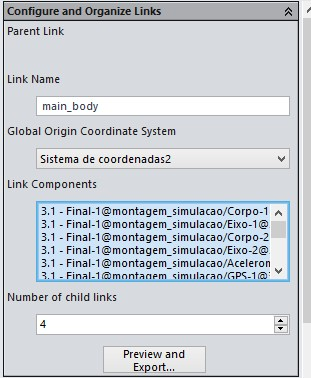
\includegraphics[scale=1]{Imagens/main_body.JPG} % aqui é onde chamamos a figura o que está entre [] são opções de formatação da figura e o que está entre {} é o nome da figura
\caption{Tela para configuração do link principal} % esta é a legenda da figura
\end{figure} % aqui acaba o ambiente figura.

Após a definição do link principal, deve-se selecionar um link filho para editar. A seleção é feita no canto inferior esquerdo, clicando-se em Emptyl\_link, como mostrado na figura abaixo.

\begin{figure}[!htb]% aqui começa o ambiente figura
\centering % este comando é para centralizar a figura
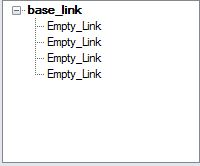
\includegraphics[scale=1]{Imagens/ArvoreVazia.JPG} % aqui é onde chamamos a figura o que está entre [] são opções de formatação da figura e o que está entre {} é o nome da figura
\caption{Tela para se iniciar a configuração de um link filho} % esta é a legenda da figura
\end{figure} % aqui acaba o ambiente figura.

Em seguida deve se editar cada link filho do modelo. Como os links filhos se movimentam, algumas informações adicionais têm que ser inseridas:

\begin{description}
\item [Link Name] é o nome dado ao link do modelo a ser exportado;
\item [Joint Name] é o nome dado a junta do modelo a ser exportado;
\item [Reference Coordinate System] é  o eixo de coordenadas que será a referência para esse link; 
\item [Reference Axis] é o eixo de referência para o movimento da junta;
\item [Joint Type] é o tipo da junta, definido pela maneira como a qual se movimenta. Pode ser por revolução, contínua, prismática ou fixa;
\item [Link Components] local onde se define quais componentes do desenho CAD farão parte do link especificado; 
\item [Number of child links] é onde se determina quantos links serão ligados ao ao link em questão;
\end{description}

\begin{figure}[!htb]% aqui começa o ambiente figura
\centering % este comando é para centralizar a figura
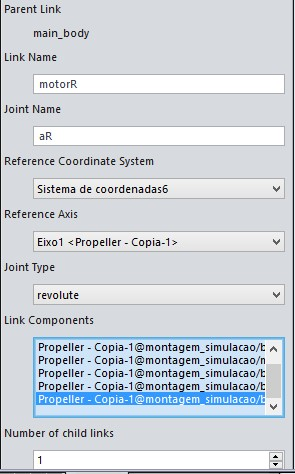
\includegraphics[scale=01]{Imagens/motorR.JPG} % aqui é onde chamamos a figura o que está entre [] são opções de formatação da figura e o que está entre {} é o nome da figura
\caption{Tela para configuração de links filhos} % esta é a legenda da figura
\end{figure} % aqui acaba o ambiente figura.

Para o VANT-3.0 foram usadas as configurações encontradas nas Tabelas \ref{tab:mainbody}, \ref{tab:servodireito}, \ref{tab:helicedireita}, \ref{tab:servoesquerdo}, \ref{tab:hélice esquerda}, \ref{tab:empenagemhorizontal} e \ref{tab:empenagemvertical}.


% Table generated by Excel2LaTeX from sheet 'Sheet1'
\begin{table}[htbp]
\centering
\begin{tabular}{|l|cccc|}
\hline
Link Name & \multicolumn{4}{c|}{ main\textbackslash{}\_body} \\
\hline
Global Origin Coordinate System  & \multicolumn{4}{c|}{Sistemas de coordenadas2} \\
\hline
\multicolumn{1}{|p{14.715em}|}{Link Components } & \multicolumn{4}{p{18.36em}|}{Todas as peças da montagem 3.1 - Final, com exceção do profundor e do leme} \\
\hline
Number of child links & \multicolumn{4}{c|}{4} \\
\hline
\end{tabular}%
\caption{Elo correspondente ao corpo principal}
\label{tab:mainbody}%
\end{table}%

% Table generated by Excel2LaTeX from sheet 'Sheet1'
\begin{table}[htbp]
\centering
\begin{tabular}{|l|c|c|c|c|}
\hline
Link Name & \multicolumn{4}{c|}{ motorR} \\
\hline
Joint Name & \multicolumn{4}{c|}{aR} \\
\hline
Reference Coordinate System  & \multicolumn{4}{c|}{Sistema de coordenadas6} \\
\hline
Reference Axis  & \multicolumn{4}{c|}{Eixo1<Propeller - Copia-1>} \\
\hline
Joint Type  & \multicolumn{4}{c|}{revolute} \\
\hline
Link Components   & \multicolumn{4}{c|}{Grupo propulsor da direita sem a hélice} \\
\hline
Number of child links  & \multicolumn{4}{c|}{1} \\
\hline
\end{tabular}%
\caption{Elo correspondente ao servo motor direito}
\label{tab:servodireito}%
\end{table}%

% Table generated by Excel2LaTeX from sheet 'Sheet1'
\begin{table}[htbp]
\centering
\begin{tabular}{|l|c|c|c|c|}
\hline
Link Name  & \multicolumn{4}{c|}{propeller\textbackslash{}\_R} \\
\hline
Joint Name  & \multicolumn{4}{c|}{thurst} \\
\hline
Reference Coordinate System   & \multicolumn{4}{c|}{Sistema de coordenadas6} \\
\hline
Reference Axis  & \multicolumn{4}{c|}{Eixo2<Propeller - Copia-1>} \\
\hline
Joint Type  & \multicolumn{4}{c|}{continuos} \\
\hline
Link Components   & \multicolumn{4}{c|}{Hélice da direita} \\
\hline
Number of child links  & \multicolumn{4}{c|}{0} \\
\hline
\end{tabular}%
\caption{Elo correspondente à helice direita}
\label{tab:helicedireita}%
\end{table}%

% Table generated by Excel2LaTeX from sheet 'Sheet1'
\begin{table}[htbp]
\centering
\begin{tabular}{|l|c|c|c|c|}
\hline
Link Name  & \multicolumn{4}{c|}{motorL} \\
\hline
Joint Name  & \multicolumn{4}{c|}{aL} \\
\hline
Reference Coordinate System   & \multicolumn{4}{c|}{Sistema de coordenadas4} \\
\hline
Reference Axis  & \multicolumn{4}{c|}{Eixo1<Propeller - Copia-2>} \\
\hline
Joint Type  & \multicolumn{4}{c|}{revolute} \\
\hline
Link Components   & \multicolumn{4}{c|}{Grupo propulsor da esquerda sem a hélice} \\
\hline
Number of child links & \multicolumn{4}{c|}{1} \\
\hline
\end{tabular}%
\caption{Elo correspondente ao servo esquerdo}
\label{tab:servoesquerdo}%
\end{table}%

% Table generated by Excel2LaTeX from sheet 'Sheet1'
\begin{table}[htbp]
\centering
\begin{tabular}{|l|c|c|c|c|}
\hline
Link Name  & \multicolumn{4}{c|}{popeller\textbackslash{}\_L} \\
\hline
Joint Name  & \multicolumn{4}{c|}{thurst} \\
\hline
Reference Coordinate System   & \multicolumn{4}{c|}{Sistema de coordenadas4} \\
\hline
Reference Axis  & \multicolumn{4}{c|}{Eixo2<Propeller - Copia-2>} \\
\hline
Joint Type  & \multicolumn{4}{c|}{continuos} \\
\hline
Link Components   & \multicolumn{4}{c|}{Hélice da esquerda} \\
\hline
Number of child links  & \multicolumn{4}{c|}{0} \\
\hline
\end{tabular}%
\caption{Elo correspondente à hélice esquerda}
\label{tab:hélice esquerda}%
\end{table}%

% Table generated by Excel2LaTeX from sheet 'Sheet1'
\begin{table}[htbp]
\centering
\begin{tabular}{|l|c|c|c|c|}
\hline
Link Name  & \multicolumn{4}{c|}{elevator} \\
\hline
Joint Name  & \multicolumn{4}{c|}{elev} \\
\hline
Reference Coordinate System   & \multicolumn{4}{c|}{Sistema de coordenadas9} \\
\hline
Reference Axis  & \multicolumn{4}{c|}{Eixo1<3.1 - Final/Montagem1-1>} \\
\hline
Joint Type  & \multicolumn{4}{c|}{revolute} \\
\hline
Link Components   & \multicolumn{4}{c|}{Profundor} \\
\hline
Number of child links  & \multicolumn{4}{c|}{0} \\
\hline
\end{tabular}%
\caption{Elo correpondente à empenagem horizontal}
\label{tab:empenagemhorizontal}%
\end{table}%

% Table generated by Excel2LaTeX from sheet 'Sheet1'
\begin{table}[htbp]
\centering
\begin{tabular}{|l|c|c|c|c|}
\hline
Joint Name  & \multicolumn{4}{c|}{rud} \\
\hline
Reference Coordinate System   & \multicolumn{4}{c|}{Sistema de coordenadas10} \\
\hline
Reference Axis  & \multicolumn{4}{c|}{Eixo2<3.1 - Final/Montagem1-1>} \\
\hline
Joint Type  & \multicolumn{4}{c|}{revolute} \\
\hline
Link Components   & \multicolumn{4}{c|}{Leme} \\
\hline
Number of child links  & \multicolumn{4}{c|}{0} \\
\hline
\end{tabular}%
\caption{Elo correspondente à empenagem vertical}
\label{tab:empenagemvertical}%
\end{table}%



\begin{figure}[!htb]% aqui começa o ambiente figura
\centering % este comando é para centralizar a figura
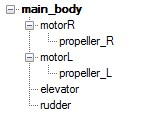
\includegraphics[scale=1.3]{Imagens/ArvoreCheia.JPG} % aqui é onde chamamos a figura o que está entre [] são opções de formatação da figura e o que está entre {} é o nome da figura
\caption{Estruturação dos links no VANT-3.0} % esta é a legenda da figura
\end{figure} % aqui acaba o ambiente figura.


Após a edição dos parâmetros deve-se clicar em 'Preview and Export...' para começar a conversão. Uma tela irá aparecer com os dados das juntas. É importante conferir os valores para assegurar um bom modelo exportado, caso em alguma junta todos os campos aparecerem em branco de ser realizada uma nova exportação. Após a verificação deve-se clicar em 'next' e realizar as mesmas conferência para os links. Não é recomendável alterar nenhum dado nessa etapa, podendo ocasionar em um modelo que não representa a realidade. Em seguida seleciona-se a opção 'Finish..' e escolhe-se a pasta adequada para salvar. As configurações ficam salvas dentro do SolidWorks® caso seja necessário repetir o processo. zz

\subsection{Modificações necessárias no projeto exportado}

\subsubsection{Adicionar arquivo config.xml} 

Adicione o subdiretório config ao produto resultante do projeto de exportação e crie o arquivo ``config.xml'' dentro do mesmo. O conteúdo deste arquivo está descrito na seção \ref{config} \\

\subsubsection{Tradução de arquivos SDF para URDF} 

O arquivo de descrição cinemática resultante do processo de exportação, que se encontra dentro do diretório \textit{urdf}, é do tipo URDF e o formato melhor adequado para uso no simulador Gazebo é o arquivo SDF. 

Antes de realizar o processo de conversão de arquivos, crie o subdiretório ``robot'', abra um novo terminal com localidade dentro do diretório do produto de exportação e utilize o seguinte comando via terminal (com devidas modificações):

\begin{bashcode}
gzsdf print urdf/oldgazeboformat.urdf > robot/model.sdf
\end{bashcode}

Posteriormente, crie o arquivo ``model.config'' dentro do diretório do projeto e preencha conforme ilustrado na figura \ref{modelconfig}

\begin{figure}[ht!]
	\begin{minted}{xml}
	<?xml version="1.0" ?>
	<model>
		<name>vant1gazebo</name>
		<version>1.0</version>
		<sdf version="1.4">robot/model.sdf</sdf>
		<author>
			<name>provant</name>
			<email>provant@hotmail.com</email>
		</author>
		<description></description>
	</model>
	\end{minted}
	\caption{Conteúdo a ser colocado no arquivo ``model.config''}
	\label{modelconfig}
\end{figure}

\chapter{Cenário}

\section{Organização}

Os arquivos associados aos cenários, utilizados no ambiente de simulação ProVANT, estão localizados na pasta referênte ao caminho:

\begin{bashcode}
$HOME/catkin\_ws/src/provant\_simulator/source/Database/worlds/worlds
\end{bashcode}

Atualmente, todos os cenários inclusos no ambiente de simulação são cenários vazios. Estes arquivos estão localizados no subdiretório 'Empty' e estão acompanhadas por um arquivo do tipo GIF para sua ilustração na interface gráfica. Estes arquivos configuram o funcionamento do simulador e a inclusão de um único modelo. 

Nesta versão á dois cenários: i) Cenário vazio com a inclusão do modelo VANT 2.0; ii) Cenário vazio com a inclusão do modelo VANT 2.0. No entanto o ambiente de simulação não se limita apenas a esses arquivos, a criação de novo cenário é descrita na próxima seção.

\section{Estrutura}

A estrtura básica de um arquivo ``.world'' está ilustrado na Figura \ref{empty.world}. Este arquivo é preenchido com tags XML e há 4 comandos principais: i) definição da aceleração da gravidade; ii) definição de configurações do motor de simulação; iii) inclusão do plugin Mundo; iv) inclusão de modelos.

\begin{figure}[ht!]
	\begin{minted}{xml}
	<?xml version="1.0" encoding="UTF-8"?>
	<sdf version="1.6">
	<world name="vant3.world">
		<gravity>0 0 -9.8</gravity>
		<physics type="simbody">
			<max_step_size>0.001000</max_step_size>
			<real_time_factor>0</real_time_factor>
		</physics>
		<plugin name="gazebo_tutorials" filename="libgazebo_ros_world_plugin.so"/>
		<include>
			<uri>model://ground_plane</uri>
			<static>false</static>
		</include>
		<include>
			<uri>model://sun</uri>
			<static>false</static>
		</include>
		<include>
			<uri>model://vant3</uri>
			<name>newmodel</name>
			<static>false</static>
			<pose>0 0 1 0 0 0</pose>
		</include>
	</world>
	</sdf>\end{minted}
	\caption{Exemplo de cenário}
	\label{empty.world}
\end{figure}


A definição da aceleração da gravidade está na tag \textcolor{blue}{<gravity></gravity>}. O primeiro elemento corresponde o módulo do componente vetorial na direção x; o segundo, em y; e o terceiro; e o terceiro, em z.

As opções do motor de simulação estão explicitadas na tag \textcolor{blue}{<physics></physics>}. Internamente, as opções configuradas são: i) \textbf{type}, que especifica qual motor de simulação será utilizado; ii) \textbf{max\_step\_size}, que define o valor do passo de simulação; e \textbf{real\_time\_factor}, que define o fator de tempo real que o simulado utilizará. Neste último, se estiver configurada com o valor 0, o passo de amostragem será executado o mais rápido possível; se 1, o passo de simulação será executado conforme o tempo real.

Para incluir um modelo no cenário utiliza-se \textcolor{blue}{<include></include>}. Neste comando, o campo \textbf{uri} especifica o modelo; \textbf{name} define o nome do modelo; \textbf{static} define se o modelo será estático, isto é, o motor de simulação relevará sua existência; e \textbf{pose} especifica a pose inicial do modelo.
	
Por fim, tem-se a inclusão de plugin Mundo por meio da tag \textcolor{blue}{<plugin></plugin>}. Nela especificamos um nome qualquer por meio de \textbf{name} e o nome do arquivo do plugin, \textbf{filename}. 


\section{Criando novo cenários}

Para criar um novo cenário, exite duas possibilidades: i) adicionar um arquivo cenário já existente (neste caso, cenário vazio), porém com outra configuração de vant; ii) criar um outro cenário.

\subsection{Adicionar um arquivo cenário já existente}

No mesmo diretório do cenário já existente, copie e cole um dos arquivos ``.worlds'' existentes de maneira a duplicar o mesmo. Modifique o nome do arquivo duplicado para um nome qualquer e altere suas configurações se desejado, por exemplo nome vant e pose inicial.

\subsection{Criar um outro cenário}

Crie um novo diretório. Internamente, crie um arquivo ``.world'' com as configurações desejadas e adicione um arquivo ``imagem.gif'' ilustrando esse cenário. Esta foto servirá para uso na interface de auxílio ao usuário.




\chapter{Plugins e sensores}

O funcionamento de um vant necessita de intrumentação para medição e atuação de variáveis físicas, por exemplo, GPS e motores. Dada essa importância, o simulador Gazebo fornece ao usuário elementos de simulação capazes ler/modificar variáveis de simulação durante a sua execução. 

Esta versão do ambiente de simulação ProVANT fornece um conjunto fixo destes elementos. Assim, com o objetivo de documentá-los e orientar, futura manutenção e desenvolvimento do ambiente de simulação, este capítulo descreve a organização e estrutura da instrumentação.

Há dois tipos de instrumentos na plataforma de simulação: i) elementos padronizados disponíveis o Gazebo de pronto para uso; ii) elementos customizados. Aqueles são denominados ``Sensores'' e o estes, `` Plugins''. 


\section{Plugins}

Plugins são bibliotecas dinâmicas criadas pelo usuário que são carregadas durante a inicialização do simulador Gazebo a partir das configurações aplicadas no arquivo de descrição de modelo ou no arquivo de descrição de cenário (arquivos SDF). Tais bibliotecas tem a capacidade de interagir com a simulação em execução, seja adquirindo dados e aplicando sinais de controle, seja alterando configurações de simulação. \\

De modo geral, o Gazebo possui 6 tipos de plugins:

\begin{enumerate}[noitemsep]
\item Mundo
\item Modelo
\item Sensor
\item Sistema
\item Visual
\item GUI
\end{enumerate}

Dentre o 6 tipos, o ambiente de simulação apenas utiliza os plugins Mundo e Modelo. O diretório com código fonte e arquivos para compilação e construção destes está em:

\begin{bashcode}
	$HOME/catkin\_ws/src/provant_simulator/source/Structure/
	custom_plugins
\end{bashcode}

No entando, o diretório com todo o código fonte está organizado no subdiretório \textbf{plugins}, conforme ilustrado na figura \ref{plugins.JPG}.

\begin{figure}[H]
\centering
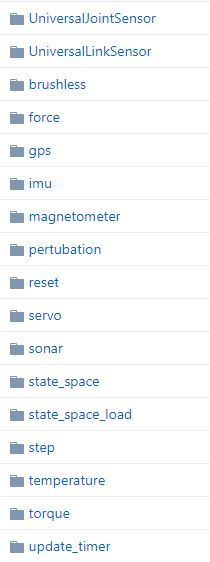
\includegraphics[width=0.45\textwidth]{figuras/plugins.JPG}
\caption{Lista de plugins}
\label{plugins.JPG}
\end{figure}

Mais detalhes leia este tutorial encontrado no site do Gazebo: \url{http://gazebosim.org/tutorials/?tut=plugins\_hello\_world}

\subsection{Plugins Modelo}

\subsubsection{Opções disponibilizadas no ambiente de simulação}

\begin{itemize}
\item Brushless
\begin{itemize}
\item[Descrição:] plugin para simulação das forças de empuxo resultado do giro das duas hélices pelos motores brushless de um tilt-rotor
\item[Arquivo:] libgazebo\_ros\_brushless\_plugin.so
\item[Configurações:]
\begin{itemize}
\item <topic\_FR> </topic\_FR> nome do tópico refente ao valor da força a ser aplicada na hélice direita
\item <topic\_FL> </topic\_FL> nome do tópico refente ao valor da força a ser aplicada na hélice esquerda
\item <topic\_FL> </topic\_FL>
\item <LinkDir> </LinkDir> Elo correspondente à hélice direita (a força será aplicada no eixo z desse elo)
\item <LinkEsq> </LinkEsq> Elo correspondente à hélice esquerda (a força será aplicada no eixo z desse elo)
\end{itemize}
\end{itemize}
\item Servo
\begin{itemize}
\item[Descrição:] plugin para simulação servo motor com funções de Torque e posição
\item[Arquivo:] libgazebo\_servo\_motor\_plugin.so
\item[Configurações]
\begin{itemize}
\item <NameOfJoint> </NameOfJoint> nome da junta a ser controlada pelo servo motor
\item <TopicSubscriber> </TopicSubscriber> nome do tópico com valores de referência para o servo motor
\item <TopicSubscriber> </TopicSubscriber>
\item <LinkDir> </LinkDir> Nome do tópico com valores de sensoriamento do servo (posição e velocidade)
\item <Modo> </Modo> Modo de funcionamento do servo motor
\end{itemize}
\end{itemize}
\item State\_space
\begin{itemize}
\item[Descrição:] plugin para sensoriamento do vetor de estados de um VANT Tilt-rotor. \\ $(x,y,z, \phi,\theta,\psi,\alpha_R,\alpha_L,\frac{dx}{dt},\frac{dy}{dt},\frac{dz}{dt}, \frac{d\phi}{dt},\frac{d\theta}{dt},\frac{d\psi}{dt},\frac{d\alpha_R}{dt},\frac{d\alpha_L}{dt})$
\item[Arquivo:] libgazebo\_AllData\_plugin.so
\item[Configurações]
\begin{itemize}
\item <NameOfTopic> </NameOfTopic> nome do tópico para o usuário obter informações
\item <NameOfJointR> </NameOfJointR> nome a junta do servo motor direito
\item <NameOfJointL> </NameOfJointL> nome a junta do servo motor esquerdo
\item <bodyname> </bodyname> nome do elo correspondente ao corpo principal do servo motor
\end{itemize}
\end{itemize}
\item State\_space\_load
\begin{itemize}
\item[Descrição:] plugin para sensoriamento do vetor de estados de um VANT Tilt-rotor com a função transporte de carga.  \\ $(x,y,z,\phi,\theta,\psi,\alpha_R,\alpha_L,\lambda_x,\lambda_y
\frac{dx}{dt},\frac{dy}{dt},\frac{dz}{dt},\frac{d\phi}{dt},\frac{d\theta}{dt},\frac{d\psi}{dt},\frac{d\alpha_R}{dt},\frac{d\alpha_L}{dt},\frac{d\lambda_x}{dt},\frac{d\lambda_y}{dt})$
\item[Arquivo:] libgazebo\_AllData2\_plugin.so
\item[Configurações]
\begin{itemize}
\item <NameOfTopic> </NameOfTopic> nome do tópico para o usuário obter informações
\item <NameOfJointR> </NameOfJointR> nome a junta do servo motor direito
\item <NameOfJointL> </NameOfJointL> nome a junta do servo motor esquerdo
\item <NameOfJoint\_X> </NameOfJoint\_X> nome a junta correspondente ao grau de liberdade da carga em torno do eixo X
\item <NameOfJoint\_Y> </NameOfJoint\_Y> nome a junta correspondente ao grau de liberdade da carga em torno do eixo Y
\item <bodyname> </bodyname> nome do elo correspondente ao corpo principal do servo motor
\end{itemize}
\end{itemize}
\item temperature
\begin{itemize}
\item[Descrição:] plugin para sensoriamento da temperatura e pressão atmosférica com ruído. \\ 
\item[Arquivo:] libgazebo\_ros\_temperature.so
\item[Configurações]
\begin{itemize}
\item <Topic> </Topic> nome do tópico para o usuário obter dados sensoriais
\item <TempOffset> </TempOffset> offset de erro para dados de temperatura ruidosos
\item <TempStandardDeviation> </TempStandardDeviation> desvio padrão  de erro para dados de temperatura ruidosos
\item <BaroOffset> </BaroOffset> offset de erro para dados de pressão ruidosos
\item <BaroStandardDeviation> </BaroStandardDeviation> desvio padrão  de erro para dados de pressão ruidosos
\item <maxtemp> </maxtemp> valor máximo de temperatura
\item <mintemp> </mintemp> valor mínimo de temperatura
\item <maxbaro> </maxbaro> valor máximo de pressão
\item <minbaro> </minbaro> valor mínimo de pressão
\item <Nbits> </Nbits> quantidade de bits utilizados na digitalização
\end{itemize}
\end{itemize}
\item UniversalJointSensor
\begin{itemize}
\item[Descrição:] plugin para sensoriamento de todos os dados que o Gazebo disponibiliza de uma junta. (ângulo,velocidade angular e Torque)\\ 
\item[Arquivo:] libgazebo\_ros\_universaljoint.so
\item[Configurações]
\begin{itemize}
\item <NameOfTopic> </NameOfTopic> nome do tópico para o usuário obter dados sensoriais
\item <NameOfJoint> </NameOfJoint> nome da junta para sensoriamento
\item <Axis> </Axis> Eixo de rotação da junta (" para primeira junta e "axis2" para segunda junta - gazebo contém juntas q permite dois graus de liberdade)
\end{itemize}
\end{itemize}
\item UniversalLinkSensor
\begin{itemize}
\item[Descrição:] plugin para sensoriamento de todos os dados que o Gazebo disponibiliza de um elo. \\
\item[Ordem de informações]
\begin{itemize}
\item pose relativa em x
\item pose relativa em y
\item pose relativa em z
\item pose relativa em $\phi$
\item pose relativa em $\theta$
\item pose relativa em $\psi$
\item velocidade relativa em x
\item velocidade relativa em y
\item velocidade relativa em z
\item aceleração linear relativa em x
\item aceleração linear relativa em y
\item aceleração linear relativa em z
\item força relativa em x
\item força relativa em y
\item força relativa em z
\item velocidade angular relativa em x
\item velocidade angular relativa em y
\item velocidade angular relativa em z
\item aceleração angular relativa em x
\item aceleração angular relativa em y
\item aceleração angular relativa em z
\item conjugado mecânico relativa em x
\item conjugado mecânico relativa em y
\item conjugado mecânico relativa em z
\item pose global em x
\item pose global em y
\item pose global em z
\item pose global em $\phi$
\item pose global em $\theta$
\item pose global em $\psi$
\item velocidade global em x
\item velocidade global em y
\item velocidade global em z
\item aceleração linear global em x
\item aceleração linear global em y
\item aceleração linear global em z
\item força global em x
\item força global em y
\item força global em z
\item velocidade angular global em x
\item velocidade angular global em y
\item velocidade angular global em z
\item aceleração angular global em x
\item aceleração angular global em y
\item aceleração angular global em z
\item conjugado mecânico global em x
\item conjugado mecânico global em y
\item conjugado mecânico global em z
\item velocidade linear do centro de gravidade global em x
\item velocidade linear do centro de gravidade global em y
\item velocidade linear do centro de gravidade global em z
\item pose linear do centro de gravidade global em x
\item pose linear do centro de gravidade global em y
\item pose linear do centro de gravidade global em z
\end{itemize}

\item[Arquivo:] libgazebo\_ros\_universallink.so
\item[Configurações]
\begin{itemize}
\item <NameOfTopic> </NameOfTopic> nome do tópico para o usuário obter dados sensoriais
\item <NameOfLink> </NameOfLink> nome da elo para sensoriamento
\end{itemize}
\end{itemize}
\end{itemize}

\subsubsection{Inserindo no arquivo de descrição do modelo}

Para inserir plugins modelos basta inserir tags <plugin></plugin>, definindo nome, nome da biblioteca dinâmica e as tags internas necessárias para configuração do plugin. O exemplo abaixo demonstra como referenciar plugins modelo no arquivo SDF. 

\begin{minted}{xml}
<?xml version="1.0" encoding="UTF-8"?>
<sdf version="1.4">
	<model name="modelo">
		<link name="corpo">
			...
		</link>
		<link name="servo">
			...
		</link>
		<joint name="corpo_servo">
			...
		</joint>
		<plugin name="1" filename="1.so">
			<config1> </config1>
			<config2> </config2>
			...
		</plugin>
		<plugin name="2" filename="2.so">
			<config3> </config3>
			<config4> </config4>
			...
		</plugin>
	</model>
</sdf>
\end{minted}

\subsubsection{Processo de criação de novo plugin Modelo}

O processo de criação de um plugin do ponto de vista de desenvolvimento de software consiste na criação de uma classe (composta por arquivos .hpp e .cpp) com interface definida préviamente. No caso, o código fonte deve herdar a interface que está definida na classe ModelPlugin. Esta classe possui três métodos virtuais que são:

\begin{itemize}
\item Init(): método referente ao comportamento personalizado de inicialização do plugin.
\item Load(): Método onde carrega as configurações definidas no arquivo XML, sobretudo ponteiros para acesso a manipulação e sensoriamento de elos e juntas.
\item Reset(): Método para o comportamento personalizado de redefinição do plugin.
\end{itemize}

Mais detalhes na classe pai ModelPlugin podem ser encontrados em \url{http://osrf-distributions.s3.amazonaws.com/gazebo/api/dev/classgazebo_1_1ModelPlugin.html}

A seguir apresenta o exemplo de um código fonte de um plugin model. Neste exemplo é demonstrado a estruturade um arquivo fonte de um plugin e mostrar como os plugins são interrompidos a todo passo de simulação. Detalhes de como programar cada método com o comportamento desejado pode ser utilizado o código fonte deste projeto e o site \url{http://osrf-distributions.s3.amazonaws.com/gazebo/api/}\\

\textbf{Arquivo Exemplo.hpp}

\begin{minted}{c++}
#include <gazebo/physics/physics.hh>
#include <gazebo/transport/TransportTypes.hh>
#include <gazebo/common/Time.hh>
#include <gazebo/common/Plugin.hh>
#include <gazebo/common/Events.hh>
#include <update_timer.h>

namespace gazebo
{
	class Exemplo : public ModelPlugin
	{		
		public: 
		virtual void Init();
		virtual void Load(physics::ModelPtr _model, sdf::ElementPtr _sdf); 
		virtual void Reset();
		
		protected: 
		virtual void Update(); 
		
		private:
		physics::WorldPtr world; 
		UpdateTimer updateTimer;
		event::ConnectionPtr updateConnection;
	};
}
\end{minted}

\textbf{Arquivo Exemplo.cpp}


\begin{minted}{c++}
#include <Exemplo.hpp>

namespace gazebo
{
	void Exemplo::Init()
	{
		// Do something when the plugins starts	
	}
	
	void Exemplo::Load(physics::ModelPtr _model, sdf::ElementPtr _sdf)
	{	
		// Loading data
		world = _model->GetWorld();	
		updateTimer.Load(world, _sdf);
		updateConnection = updateTimer.Connect(boost::bind(&Exemplo::Update, this));
	}
	
	void ServoMotorPlugin::Reset()
	{
		// Do something when reset
	}
	
	void ServoMotorPlugin::Update()
	{
		// Do some something in each simulation time
			
	}
	
	GZ_REGISTER_MODEL_PLUGIN(Exemplo)
}
\end{minted}

Os métodos \textit{Init}, \textit{Load} e \textit{Reset}, como já explicado, realizam, respectivamente comandos de inicilização, leitura de informações do arquivo SDF e reset de simulação. Já o método \textit{Update}, não se encontra na interface do plugin pai \textit{ModelPlugin}, mas é um método que é configurado para ser chamado a todo momento que ocorrer um passo de simulação do Gazebo.

Essa configuração ocorre dentro do método \textit{Load}. Este obtém o ponteiro \textit{\_model} para dados do arquivo SDF do modelo e através do método do conteúdo deste ponteiro \textit{GetWorld}, ele obtém o ponteiro para a estrtura de dados com as informações do cenário. Posteriormente, este estrutura é carregada na classe \textit{UpdateTimer} e é realizado a sua inicialização. Esta estrtura que informa a necessidade de ocorrências de interrupções a cada passos de simulação. 

\subsection{Plugins Mundo}

Um preocupação neste trabalho foi garantir a sincronização entre Controlador (que será descrito posteriormente) e a simulação, conforme ilustrado na figura \ref{flow.jpg}. De forma sequencial os subsistemas serão executados e quando um sistema está executando os outros estão em repouso. Iniciamente, acontece um passo de simulação no Gazebo, os sensores obtém dados do ambiente e manda-os para tópicos de sensores. Em seguida os controladores serão avisados que chegou dados nestes tópicos, assim computará sua lei de controle e enviará os sinais de controle obtidos para tópicos de conexão com atuadores. Por fim os atuadorestrasnmitirão os sinais de controle para o amabiente de simulação.


\begin{figure}[H]
\centering
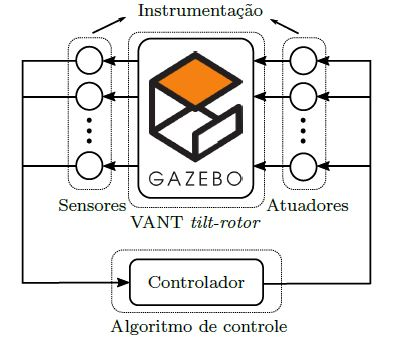
\includegraphics[width=0.65\textwidth]{figuras/flow.jpg}
\caption{Esquemático do simulador}
\label{flow.jpg}
\end{figure}


O controlador é um executável que somente é executado quando chegar novos dados de sensores, no entanto, o Gazebo já é configurado por padrão de rodar indefinidamente. Então com a finalidade de garantir que os componentes do sistem executem sequencialmente, propou-se em deixar o simulador em suspensão e quando necessitar o controlador solicita a execução de novo passo de simulação. Para possibilitar a comunicação do controlador e simulador nesse sentido, projetou-se um plugin mundo que através de uma conxão externa através de tópicos do ROS possibilita que o controlador comande a execução do momento necessário para a execução de novo passo de simulação.

A configuração do plugin mundo é definida como:

\begin{itemize}
\item Step plugin
\begin{itemize}
\item[Descrição:] plugin comando externo do Controlador para solicitação de novo passo de simulação
\item[Arquivo:] libgazebo\_ros\_world\_plugin.so
\item[Configuração:] Nome do tópico definido permanentemente como Step
\end{itemize}
\end{itemize}

\section{Sensores disponíveis}

O sensores, diferentemente dos plugins modelo, são implementados pelo próprio Gazebo e, após serem referenciados no arquivo de descrição do modelo, disponibilizam os seus dados por meio de tópicos do Gazebo. Estes tópicos funcionam semelhantemente aos tópicos do Gazebo, porém possui API própria para lidar com a escrita e leitura de dados. Veja mais detalhes em \url{http://www.robopgmr.com/?p=5614}.

No entanto, como os tópicos do ROS e GAzebo não possuem conexão, é necessário fazer trasnmissão de dados entre ambas as tecnologias de comunicação entre processos. Essa comunicação foi feita, desenvolvendo plugins modelos apenas com essa função. Aqui chamaremos de conversores de dados.

\subsubsection{Opções disponibilizadas}

Diversos são os sensores disponibilizados pelo Gazebo e sua configuração no arquivo SDF estão descritas em \url{http://sdformat.org/spec?ver=1.6&elem=sensor}. Porém apenas alguns coversores de dados foram desenvolvidos para esta versão e são GPS, Sonar, Magnetômetro, IMU. Suas configurações são:

\begin{itemize}
\item GPS
\begin{itemize}
\item[Descrição:] plugin para conversão e transporte de dados entre plugins Gazebo e ROS
\item[Arquivo:] libgazebo\_ros\_sonar.so
\item[Configurações:]
\begin{itemize}
\item <gazebotopic> </gazebotopic> nome do tópico Gazebo
\item <rostopic> </rostopic> nome do tópico ROS
\item <link> </link> nome do elo que o sensor está acoplado
\end{itemize}
\end{itemize}
\end{itemize}

\begin{itemize}
\item Sonar
\begin{itemize}
\item[Descrição:] plugin para conversão e transporte de dados entre plugins Gazebo e ROS
\item[Arquivo:] libgazebo\_ros\_sonar.so
\item[Configurações:]
\begin{itemize}
\item <gazebotopic> </gazebotopic> nome do tópico Gazebo
\item <rostopic> </rostopic> nome do tópico ROS
\item <link> </link> nome do elo que o sensor está acoplado
\end{itemize}
\end{itemize}
\end{itemize}

\begin{itemize}
\item Magnetômetro
\begin{itemize}
\item[Descrição:] plugin para conversão e transporte de dados entre plugins Gazebo e ROS
\item[Arquivo:] libgazebo\_ros\_magnetometer.so
\item[Configurações:]
\begin{itemize}
\item <gazebotopic> </gazebotopic> nome do tópico Gazebo
\item <rostopic> </rostopic> nome do tópico ROS
\item <link> </link> nome do elo que o sensor está acoplado
\end{itemize}
\end{itemize}
\end{itemize}

\begin{itemize}
\item IMU
\begin{itemize}
\item[Descrição:] plugin para conversão e transporte de dados entre plugins Gazebo e ROS
\item[Arquivo:] libgazebo\_ros\_imu.so
\item[Configurações:]
\begin{itemize}
\item <gazebotopic> </gazebotopic> nome do tópico Gazebo
\item <rostopic> </rostopic> nome do tópico ROS
\item <link> </link> nome do elo que o sensor está acoplado
\end{itemize}
\end{itemize}
\end{itemize}

\subsubsection{Inserindo Sensor e conversor no arquivo de descrição de modelo}

Nesta parte será ilustrado como inserir um sensor com seu respectivo conversor de dados no arquivo modelo.





%\chapter{Plugins}

% Introdução de plugins

\section{Localização no projeto}

\section{Plugins modelos disponíveis}

\section{Sensores disponíveis}
\chapter{Controlador}

Este capítulo descreve o Controlador. Este é um software projetado para controlar a simulação garantindo sincronia com o Gazebo. Inicialmente, é descrito a localização de seus componente no projeto e a arquitetura de software utilizada.e seus arquivos de configuração. Em seguida, será exposto como é realizado a sua configuração e o processo de comunicação com os plugins do Gazebo. Por fim, é especificado os plugins de controle existentes, o processo de criação de novos plugins de controle e o processo de armazenamento de dados de simulação.

\section{Localização no projeto}


\textbf{\emph{Controller}}
\vspace{0.5em}

A figura \ref{fig:arvore_controller} ilustra o diretório \emph{Controller}.

\begin{tiny}
	\begin{figure}[htbp]
		\begin{forest}
			for tree={font=\sffamily, grow'=0,
				folder indent=.9em, folder icons,
				edge=densely dotted}
			[Controller
			[include
			]
			[src
			]
			[CMakeLists.txt
			]
			[package.xml
			]
			]
		\end{forest}
		\caption{Árvore do diretório \emph{Controller}.}
		\label{fig:arvore_controller}
	\end{figure}
\end{tiny}

\vspace{0.5em}
\noindent 
\textbf{\emph{control\_strategies}}
\vspace{0.5em}

A figura \ref{fig:arvore_control} ilustra o diretório \emph{control\_strategies}.

\begin{tiny}
	\begin{figure}[htbp]
		\begin{forest}
			for tree={font=\sffamily, grow'=0,
				folder indent=.9em, folder icons,
				edge=densely dotted}
			[control\_strategies
			[vant2load\_hinfinity
			]
			[vant2\_lqr
			]
			[vant3\_adaptiveMixCtrl
			]
			[vant3\_lqr
			]
			[vantloadMarcelo
			]
			[lcontroller.hpp, is file]
			]
		\end{forest}
		\caption{Árvore do diretório \emph{control\_strategies}.}
		\label{fig:arvore_control}
	\end{figure}
\end{tiny}

\vspace{0.5em}
\noindent 
\textbf{\emph{custom\_plugins}}
\vspace{0.5em}

A figura \ref{fig:arvore_customplugins} ilustra o diretório \emph{custom\_plugins}.

\begin{tiny}
	\begin{figure}[htbp]
		\begin{forest}
			for tree={font=\sffamily, grow'=0,
				folder indent=.9em, folder icons,
				edge=densely dotted}
			[custom\_plugins
			[include
			]
			[src
			]
			[plugins
			]
			[CMakeLists.txt
			]
			[package.xml
			]
			]
		\end{forest}
		\caption{Árvore do diretório \emph{custom\_plugins}.}
		\label{fig:arvore_customplugins}
	\end{figure}
\end{tiny}

\vspace{0.5em}
\noindent 
\textbf{\emph{Matlab}}
\vspace{0.5em}

A figura \ref{fig:arvore_matlab} ilustra o diretório \emph{Matlab}.

\begin{tiny}
	\begin{figure}[htbp]
		\begin{forest}
			for tree={font=\sffamily, grow'=0,
				folder indent=.9em, folder icons,
				edge=densely dotted}
			[Matlab
			[erro.txt, is file]
			[in.txt, is file]
			[out.txt, is file]
			[ref.txt, is file]
			]
		\end{forest}
		\caption{Árvore do diretório \emph{Matlab}.}
		\label{fig:arvore_matlab}
	\end{figure}
\end{tiny}

\vspace{0.5em}
\noindent 
\textbf{\emph{simulator\_msgs}}
\vspace{0.5em}

A figura \ref{fig:arvore_matlab} ilustra o diretório \emph{Matlab}.

\begin{tiny}
	\begin{figure}[htbp]
		\begin{forest}
			for tree={font=\sffamily, grow'=0,
				folder indent=.9em, folder icons,
				edge=densely dotted}
			[Matlab
			[msg]
			[CMakeLists.txt, is file]
			[package.xml, is file]
			]
		\end{forest}
		\caption{Árvore do diretório \emph{simulador\_msgs}.}
		\label{fig:arvore_simuladormsgs}
	\end{figure}
\end{tiny}

\section{Arquivo config.xml}

\label{config}



\section{Arquitetura de Software}


\subsection{Tópicos e mensagens do ROS entre Controlador e Sensores/Plugins}

Sensores/plugins com função sensorial comunicam com o Gazebo através de tópicos com mensagens padronizadas denominadas \textit{Sensor}. Como estas mensagens podem chegar com ordens indefinidas, existe uma lógica no controlador que ordena uma estrtura denominada SensorArray de acordo com uma ordem previamente estabelecida pelo usuário através de um arquivo XML. Assim, quando o usuário projetar um novo controlador, ele terá acesso a um vetor de sensores conforme desejado. Isto está ilustrado na Figura \ref{Msgs1.jpg}.


\begin{figure}[H]
	\centering
	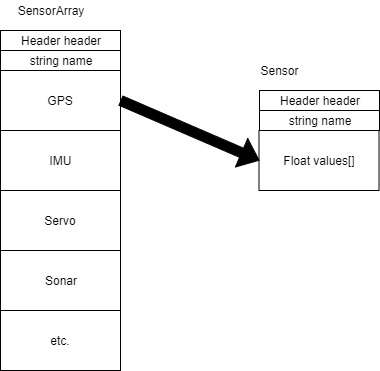
\includegraphics[width=0.65\textwidth]{figuras/Msgs1.jpg}
	\caption{Mensagens utilizadas para comunicação entre Gazebo e Simulador}
	\label{Msgs1.jpg}
\end{figure}

Além disso, a comunicação entre controlador e plugins ocorre por meio de tópicos com mensagens correspondendo a pontos flutuantes valores. Mais detalhes, o código se encontra auto-explicativo.  


\chapter{Interface Gráfica}

\section{Localização no projeto}

\section{Arquitetura de Software}



\chapter{Instalando e Compilando projeto}

Este capítulo explica o processo de instalação e compilação do projeto. No entanto, para entender o assunto é necessário introduzir conhecimento prévio sobre sistema operacional Linux e a interface Shell. Além disso, é necessário conhecimento prévio de ROS e QT que, por sua vez, foram introduzidos nos capítulos x e y. 

\section{Introdução ao linux}

Sistema operacional é o conjunto de programas que gerenciam recursos, processadores, dispositivos de entrada e saída e seus periféricos. Ele permite a comunicação entre o hardware e os demais softwares. Exemplos: Dos, Unix, Linux, Mac OS, OS-2, Windows NT. \cite{SisOp}

No contexto de plataformas Linux, o termo Linux denomina o núcleo do sistema operacional, responsável pela comunicação entre hardware e software do computador. No entanto, também é necessário outros programas para a interação entre usuário e kernel, por exemplo: compilador e a interface gráfica. Ou seja, no contexto de plataforma Linux, um sistema operacional é o conjunto do kernel e demais programas. 

Existe diversos sistemas operacionais que utilizam o kernel Linux, diferenciando-se entre si apenas das ferramentas disponíveis para interação o usuário e kernel. Cada conjunto de ferramentas e kernel é denominado distribuição e os alguns exemplos são Debian, Ubuntu e openSUSE. Apesar da diferença, não se pode distinguir qual melhor distribuição, mas sim afirmar qual delas se adequa melhor à alguma tarefa de interesse.Mais informações pode ser obtidas em \cite{Linux}

\section{Shell}

Uma das ferramentas disponíveis para a interação entre usuário e kernel é denominado Shell. Este é um programa criado com o intuito de interpretar comandos passados pelo usuário. Na verdade,  ele é um arquivo executável, encarregado de interpretar comandos passados através de um conjunto de caracteres, transmití-los ao sistema e devolver resultados.
 
Quando se executa um comando, existe 3 tipos fluxos de informação, conforme é demonstrado na figura \ref{fluxo_shell} e estão descritos a seguir

\begin{itemize}
	\item \textbf{stdin}, do inglês ''standard input``, é o fluxo de dados de entrada. Por padrão, o stdin se refere ao teclado e é identificado pelo número 0;
	\item \textbf{stdout}, do inglês ''standard output``, é o fluxo de dados de saída. Por padrão, o stdout se refere à tela e é identificado pelo número 1;
	\item \textbf{stderr}, do inglês ''standard error``, é o fluxo de mensagens de erro. Por padrão, o stderr se refere à tela e é identificado pelo número 2: 
\end{itemize}

\begin{figure}[H]
	\centering
	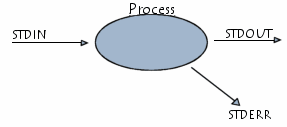
\includegraphics[width=0.65\textwidth]{variaveis/fluxo_shell.jpg}
	\caption{Fluxos de entrada e saída durante a execução de um comando. Imagem obtida de \cite{Shell}}
	\label{fluxo_shell}
\end{figure}



Por padrão, quando se executa um programa, os dados são lidos a partir do teclado e o programa envia a sua saída e os seus erros para a tela. No entanto, também é possível ler os dados a partir de qualquer dispositivo de entrada, ou mesmo a partir de um arquivo, e enviar a saída para um dispositivo de visualização, arquivo etc. Mais informações podem ser obtidas em \cite{Shell}

\section{Compilando e instalando projeto de software}

O Shell, como já explicado, possui a função de executar comandos. Com a finalidade de automatizar a execução de um certo conjunto de comandos, existe disponível no ambiente Linux a ferramenta shell script. Segundo \cite{script}, ''um shell script permite encadear comandos para solucionar tarefas mais complexas, como automatizar backups, redimensionar um lote de fotografias, limpar erros de um arquivo de texto, etc. Mas eles não são apenas uma simples sequência de comandos e podem usar características comuns às linguagens de programação, como condições (if-then-else) e até loops (for, repeat)``.

Neste projeto, criou-se dois shell scripts denominados \textit{build.sh} e \textit{install.sh}. O primeiro, possui a funcionalidade de compilar todo o código fonte já descrito nos capítulos anteriores do ProVANT Simulator. Já o segundo, além de compilar o projeto, ele cria e registra variáveis de ambiente locais (serão descritas na próxima seção) e cria um link simbólico para fácil execução do sistema via terminal. Detalhes sobre os comandos utilizados nos scripts estão explicitados nos mesmos através de comentários.

\section{Variáveis de ambiente}

As variáveis de ambiente são espaços de memória responsáveis por armazenar informações pontuais do sistema. As variáveis podem ser variáveis locais ou variáveis globais. Os nomes das variáveis podem ser constituídos de quaisquer caracteres alfanuméricos (\cite{VE2}). 

Um caso representativo da importância das variáveis de ambiente é o caso da variável de ambiente PATH. A variável PATH é utilizado muitas vezes para se registrar a localização de arquivos executáveis permitindo que o usuário e outros programas possam usufruir de suas funcionalidades.

No caso do ProVANT Simulator, utiliza-se as variáveis de ambiente do ROS e as variáveis de ambiente próprias criadas durante a instalação do sistema. Nesta seção será explicitada apenas sobre as variáveis de ambiente customizadas, sendo que detalhes sobre as variáveis de ambiente do ROS podem ser encontradas em na pagina \url{http://wiki.ros.org}. 

As seguintes variáveis foram criadas:

\begin{itemize}
	\item \textbf{PROVANT\_ROS}: Diretório onde está localizado o código fonte do espaço de de trabalho do usuário no ROS
	\item \textbf{TILT\_PROJECT}: Diretório onde está todo o projeto do ProVANT Simulator 
	\item \textbf{TILT\_STRATEGIES}: Diretório onde está localizado as bibliotecas dinâmicas compiladas com as estratégias de controle de ambiente de simulação
    \item \textbf{TILT\_MATLAB} Diretório onde os arquivos com dados da simulação são
    armazenados
    \item \textbf{PROVANT\_DATABASE}: Diretório onde se encontra os arquivos de descrição de modelos e cenários
    \item \textbf{GAZEBO\_MODEL\_PATH}: Este é uma exceção, não é uma variável ambiente criado, mas sim a atualização de uma variável ambiente do Gazebo. Aqui se encontram os modelos dos VANTs para serem adicionados em simulação.	
\end{itemize}


\bibliography{telefonia/variaveis}
\chapter{Inicialização}

\section{Nós}

\section{Roslaunch}

\subsection{Localização no projeto}

\chapter{Compilando projeto}

\chapter{Variáveis de ambiente}



\appendix




\chapter{CMakeLists.txt}
\label{cmake}

Esta seção foi extraída da página \url{http://wiki.ros.org/catkin/CMakeLists.txt} no dia 25/08/2017, visite-a para mais informações.

\section{Visão geral e estrutura do arquivo CMakeLists.txt}

O arquivo CMakeLists.txt armazena comandos de compilação e instalação de pacotes de software. Necessariamente, o arquivo \textbf{deve seguir formato e a ordem a seguir}. 

\begin{enumerate}
	\setlength{\itemsep}{1pt}
	\setlength{\parskip}{0pt}
	\setlength{\parsep}{0pt}
	\item Versão CMake necessária (cmake\_minimum\_required)
	\item Nome do pacote (project())
	\item Encontrar outros pacotes CMake/Catkin necessários para compilação (find\_package())
	\item Habilitação de suporte para módulos Python (catkin\_python\_setup())
	\item Geradores de Mensagens/Serviços/Ações do ROS (add\_message\_files(), add\_service\_files(), add\_action\_files())
	\item Invocar geração de Mensagem/Serviço/Ação (generate\_messages())
	\item Especificar pacote  de compilação, informação e exportação (catkin\_package())
	\item Bibliotecas/Executáveis para compilação (add\_library()/add\_executable()/target\_link\_libraries())
	\item Testes de construção (catkin\_add\_gtest())
	\item Regras de instalação (install())	
\end{enumerate}

\section{Versão CMake}

Todo arquivo CMakeLists.txt deve começar com a declaração da versão do sistema. A versão requisitada é a 2.8.3 ou superior.

\begin{minted}{xml} 
cmake_minimum_required(VERSION 2.8.3)
\end{minted}

\section{Nome do Pacote}

O próximo item corresponde ao o nome do pacote do ROS. No exemplo a seguir, o pacote é chamado \textit{robot\_brain}.

\begin{minted}{xml} 
project(robot_brain)
\end{minted}

Obs.: Após esse comando, é possível fazer referência do nome do projeto em qualquer outro lugar através do uso da variável \${PROJECT\_NAME}.

\section{Encontrando dependências de pacotes CMake}

É necessário especificar quais outros pacotes que precisam ser localizados para compilar o projeto. Essa especificação é realizada com o comando find\_package e sempre há ao menos uma dependência pelo pacote catkin:

\begin{minted}{xml} 
find_package(catkin REQUIRED)
\end{minted}

Se o projeto depende de outros pacotes, eles são convertidos automaticamente em componentes do sistema catkin. Em vez de usar o comando  find\_package naqueles pacotes, é possível especificá-los como componentes para melhorar a legibilidade do script. O exemplo a seguir utiliza pacote 'nodelet'' como componente.

\begin{minted}{xml} 
find_package(catkin REQUIRED COMPONENTS nodelet)
\end{minted}

Obs: É necessário usar somente o comando find\_package para encontrar componentes. Não deve-se adicionar dependência de tempo de execução.

\subsection{O find\_package()}

Se um pacote é localizado através do comando find\_package, então resultará na criação de várias variáveis de ambiente do script CMakeLists que fornecem informação sobre o pacote encontrado. As variáveis de ambiente descrevem onde os arquivos dos pacotes exportados estão, quais bibliotecas o pacote depende e os caminhos destas bibliotecas. Os nomes seguem a convenção <PACKAGE NAME>\_<PROPERTY>:

\begin{itemize}
	\setlength{\itemsep}{1pt}
	\setlength{\parskip}{0pt}
	\setlength{\parsep}{0pt}
	\item[]<NAME>\_FOUND - configurado como verdadeiro caso a biblioteca é encontrada, caso contrário, falso
	\item[]<NAME>\_INCLUDE\_DIRS ou <NAME>\_INCLUDES - Caminhos de inclusão exportados pelo pacote
	\item[]<NAME>\_LIBRARIES ou <NAME>\_LIBS - Bibliotecas exportadas pelo pacote
	\item[]<NAME>\_DEFINITIONS - Definições exportadas pelo pacote
\end{itemize}


\subsection{Por que os pacotes são especificados como componentes?}

Pacotes não são realmente componentes catkin. Em vez disso, a característica de componentes foi utilizada no desenvolvimento do script para economizar tempo de digitação significativo.

Para pacotes, será vantajoso utilizar o comando find\_package para encontrá-los como componentes. Eles estão em um conjunto de variáveis criado com o prefixo catkin\_. Por exemplo, quando você estiver usando um pacote denominado ''nodelet'' no seu código, sugere-se utilizar:

\begin{minted}{xml} 
find_package(catkin REQUIRED COMPONENTS nodelet)
\end{minted}

Isto significa que os caminhos incluídos, bibliotecas, etc. exportados pelo pacote ''nodelet'' são também anexadas às variáveis catkin\_. Por exemplo, catkin\_INCLUDE\_DIRS contém os caminhos de inclusão não somente para pacote catkin mas também para para o pacote ''nodelet''. 

Podemos de maneira alternativa achar o pacote ''nodelet'' com o comando:

\begin{minted}{xml} 
find_package(nodelet)
\end{minted}

Isto significa que os caminhos, bibliotecas e demais características do pacote ''nodelet'' não seriam adicionados às variáveis catkin\_ . O que resulta em nodelet\_INCLUDE\_DIRS, nodelet\_LIBRARIES, e etc. 

As mesmas variáveis também são criadas usando

\begin{minted}{xml} 
find_package(catkin REQUIRED COMPONENTS nodelet)
\end{minted}

\subsection{Boost}

Caso esteja usando C++ e Boost, você necessita de invocar o comando find\_package() para Boost e especificar quais aspectos da Boost que você está usando como componentes. Por exemplo, se você quiser usar threads da biblioteca Boost, você utilizaria o seguinte comando:

\begin{minted}{xml} 
find_package(Boost REQUIRED COMPONENTS thread)
\end{minted}

\section{catkin\_package()}

O comando catkin\_package() especifica informações do sistema catkin para o compilador.

Esta função deve ser utilizada antes de declarar quaisquer alvos com comandos add\_library() ou add\_executable(). A função tem 5 argumentos opcionais:

\begin{itemize}
	\setlength{\itemsep}{1pt}
	\setlength{\parskip}{0pt}
	\setlength{\parsep}{0pt}
	\item[]INCLUDE\_DIRS - Caminhos de inclusão exportados pelo pacote
	\item[]LIBRARIES - Bibliotecas exportadas do projeto
	\item[]CATKIN\_DEPENDS - Outros projetos catkin que este projeto depende
	\item[]DEPENDS - Projetos não-catkin que este projeto depende
	\item[]CFG\_EXTRAS - Opções de configuração adicional
\end{itemize}

Observe o exemplo:

\begin{minted}{xml} 
catkin_package(INCLUDE_DIRS include
LIBRARIES \${PROJECT_NAME}
CATKIN_DEPENDS roscpp nodelet
DEPENDS eigen opencv)
\end{minted}

Isto indica que o diretório "include" dentro do diretório do pacote é o local que os cabeçalhos serão direcionados. A variável de ambiente \${PROJECT\_NAME} avalia informação passada para a função project(), neste caso será ''robot\_brain''. ''roscpp'' e ''nodelet'' são pacotes que necessitam estar presentes durante a compilação/execução deste pacote, já ''eigen'' e ''opencv'' são dependências do sistema que necessitam estar presentes para compilação/execução deste pacote.

\section{Especificando alvos de compilação}

Construir alvos pode ser realizadas de diversas formas, mas normalmente representam um das duas possibilidades:

\begin{itemize}
	\setlength{\itemsep}{1pt}
	\setlength{\parskip}{0pt}
	\setlength{\parsep}{0pt}
	\item[]Executable Target - programas a serem executados
	\item[]Library Target - bibliotecas que podem ser usadas por alvos executáveis durante a compilação e/ou tempo de execução
\end{itemize}

\subsection{Nomeando alvos}

É muito importante notar que os nomes dos alvos de compilação no sistema catkin devem ser únicos sem considerar os diretórios que eles foram compilados/instalados. Este é um requisito do CMake. Entretanto, nomes únicos são apenas necessários internamente para CMake. Alguém pode obter um alvo renomeado como outro nome usando o comando set\_target\_properties():

Exemplo:

\begin{minted}{xml}
set_target_properties(rviz_image_view
PROPERTIES OUTPUT_NAME image_view
PREFIX "")
\end{minted}

Isto irá trocar o nome do alvo rviz\_image\_view para image\_view na compilação e instalação de saídas.

\subsection{Diretório customizado de saída}

Enquanto o diretório de saída padrão para executáveis e bibliotecas é comum a um valor razoável, ele deve ser personalizado em certos casos. Isto é, uma biblioteca contendo ligações de Python deve ser realocada em um diretório diferente a fim de ser importável no Python.:

Exemplo:

\begin{minted}{xml}
set_target_properties(python_module_library
PROPERTIES LIBRARY_OUTPUT_DIRECTORY ${CATKIN_DEVEL_PREFIX}${CATKIN_PACKAGE_PYTHON_DESTINATION})
\end{minted}

\subsection{Caminhos de inclusão e caminhos de bibliotecas}

Antes de especificar alvos, você precisa especificar onde os recursos como arquivos de cabeçalho e bibliotecas podem ser localizados:

\begin{itemize}
	\setlength{\itemsep}{1pt}
	\setlength{\parskip}{0pt}
	\setlength{\parsep}{0pt}
	\item[]Caminhos de inclusão  
	\item[]Caminhos de biblioteca
	\item[]include\_directories(<dir1>, <dir2>, ..., <dirN>)
	\item[]link\_directories(<dir1>, <dir2>, ..., <dirN>)
\end{itemize}

\textbf{a) include\_directories()} \\

O argumento para o comando include\_directories deve ser as variáveis \_INCLUDE\_DIRS  geradas pelo chamada do comando find\_package e qualquer diretório adicional que necessita ser incluído. Se você estiver usando o sistema catkin e Boost, a chamada de include\_directories() deve ser parecer:

\begin{minted}{xml}
include_directories(include ${Boost_INCLUDE_DIRS} ${catkin_INCLUDE_DIRS})
\end{minted}

O primeiro argumento ''include'' indica que o diretório include dentro do pacote faz parte também da caminho. \\

\textbf{b) link\_directories()} \\

O comando link\_directories() pode ser usada para adicionar novos caminhos de bibliotecas, no entanto, isto não é recomendado. Todos os pacotes catkin e CMake automaticamente tem sua informação de ligação adicionado quando são encontrados pelo find\_package. 
Basta ligar as bibliotecas no target\_link\_libraries()

Exemplo:

\begin{minted}{xml}
link_directories(~/my_libs)
\end{minted}

\subsection{Alvos executáveis}

Para especificar um alvo executável que deve ser construído, deve-se usar o comando CMake add\_executable().

\begin{minted}{xml}
add_executable(myProgram src/main.cpp src/some_file.cpp src/another_file.cpp)
\end{minted}

Isto irá construir um alvo executável denominado "myProgram" que, por sua vez, é constituídos de 3 arquivos fonte: src/main.cpp, src/some\_file.cpp e src/another\_file.cpp.

\subsection{Alvos de bibliotecas}

O comando CMake add\_library() é usado para especificar bibliotecas para serem construídas. Por padrão o sistema catkin constrói bibliotecas dinâmicas.

\begin{minted}{xml}
add_library(${PROJECT_NAME} ${${PROJECT_NAME}_SRCS})
\end{minted}

\subsection{target\_link\_libraries}

Use o comando target\_link\_libraries() para especificar quais bibliotecas um alvo executável é ligado. Isto é feito tipicamente depois da chamada add\_executable(). Adicione \$\{catkin\_LIBRARIES\} se o ROS não for encontrado.

Sintaxe:

\begin{minted}{xml}
target_link_libraries(<executableTargetName>, <lib1>, <lib2>, ... <libN>)
\end{minted}

Exemplo:

\begin{minted}{xml}
add_executable(foo src/foo.cpp)
add_library(moo src/moo.cpp)
target_link_libraries(foo moo)  -- This links foo against libmoo.so
\end{minted}

Observe que não há necessidade para uso de link\_directories() na maioria dos casos, pois a informação é automaticamente enviada via find\_package().

\section{Mensagens alvos, Serviços alvos e Ações alvos}

Arquivos de mensagens (.msg), serviços (.srv), e ações (.action) no ROS requerem um passo de construção especial antes de serem construídas e usadas por pacotes do ROS. O objetivo destas macros é gerar arquivos de linguagem específica de programação de maneira que alguém utilize mensagens, serviços e ações na linguagem de programação desejada. O sistema de compilação gerará ligações usando todos os geradores disponíveis (ex. gencpp, genpy, genlisp, etc).

Estas são três macros fornecidos para tratar de mensagens, serviços e ações respectivamente:

\begin{minted}{xml}
add_message_files
add_service_files
add_action_files
\end{minted}

Estas macros devem ser seguidas por uma chamada que invoca a geração:

\begin{minted}{xml}
generate_messages()
\end{minted}

\subsubsection{Restrições/Pré-requisitos importantes}

Estas macros devem vir antes do comando catkin\_package() para correta geração.

\begin{minted}{xml}
find_package(catkin REQUIRED COMPONENTS ...)
add_message_files(...)
add_service_files(...)
add_action_files(...)
generate_messages(...)
catkin_package(...)
...
\end{minted}

O comando catkin\_package() deve ter dependência (CATKIN\_DEPENDS) do pacote message\_runtime.

\begin{minted}{xml}
catkin_package(
...
CATKIN_DEPENDS message_runtime ...
...)
\end{minted}

Você deve usar find\_package() para o pacote message\_generation, seja sozinho ou como um componente do sistema catkin:

\begin{minted}{xml}
find_package(catkin REQUIRED COMPONENTS message_generation)
\end{minted}

Seu arquivo package.xml deve conter uma dependência de construção do message\_generation e uma dependência de tempo de execução message\_runtime. Isso não é necessário se as dependências forem puxadas indiretamente de outros pacotes.
Se você tem um alvo que (mesmo indiretamente) depende de algum outro alvo que precise de mensagens/serviços/ações a serem construídas, você precisa adicionar uma dependência explícita no alvo catkin\_EXPORTED\_TARGETS, para que eles sejam construídos na ordem correta. Este caso aplica-se quase sempre, a menos que seu pacote realmente não use nenhuma parte do ROS. Infelizmente, essa dependência não pode ser propagada automaticamente. (some\_target correspondem ao nome do alvo definido por add \_executable()):

\begin{minted}{xml}
add_dependencies(some_target ${catkin_EXPORTED_TARGETS})
\end{minted}

Se você tem um pacote que cria mensagens e/ou serviços, bem como executáveis que usam estes, você precisa criar uma dependência explícita no alvo da mensagem gerada automaticamente para que eles sejam construídos na ordem correta. (some\_target correspondem ao nome do alvo definido por add\_executable ()):

\begin{minted}{xml}
add_dependencies(some_target ${${PROJECT_NAME}_EXPORTED_TARGETS})
\end{minted}

Se o seu pacote satisfizer as duas condições acima, você precisa adicionar ambas as dependências, ou seja:

\begin{minted}{xml}
add_dependencies(some_target ${${PROJECT_NAME}_EXPORTED_TARGETS} ${catkin_EXPORTED_TARGETS})
\end{minted}

\subsection{Exemplo}

Suponha que o seu pacote tenha duas mensagens em um diretório chamado "msg" chamadas "MyMessage1.msg" e "MyMessage2.msg" que dependem de std\_msgs e sensor\_msgs. Além disso, possui um serviço em um diretório chamado "srv" chamado "MyService.srv". O pacote define um executável que usa essas mensagens e serviços e um executável que usa algumas partes do ROS, mas não mensagens/serviços definidos neste pacote. Tal exemplo precisará do seguinte CMakeLists.txt:

\begin{minted}{xml}
# Obter informação sobre as dependências de compilação do pacote
find_package(catkin REQUIRED
COMPONENTS message_generation std_msgs sensor_msgs)

# Declaras arquivos mensagens para serem construídos
add_message_files(FILES
MyMessage1.msg
MyMessage2.msg
)

# Declara arquivos de serviços a serem construídos
add_service_files(FILES
MyService.srv
)

# Gera as mensagens e serviços com as linguagems específica de programação
generate_messages(DEPENDENCIES std_msgs sensor_msgs)

# Declara as dependências de tempo de execução do pacote
catkin_package(
CATKIN_DEPENDS message_runtime std_msgs sensor_msgs
)

# Define executáveis que usam mensagens.
add_executable(message_program src/main.cpp)
add_dependencies(message_program ${${PROJECT_NAME}_EXPORTED_TARGETS} ${catkin_EXPORTED_TARGETS})

# Define executável que não utiliza quaisquer mensagens/serviços fornecidos pelo pacote
add_executable(does_not_use_local_messages_program src/main.cpp)
add_dependencies(does_not_use_local_messages_program ${catkin_EXPORTED_TARGETS})
\end{minted}

Além disso, se você quer criar ações e tenha um arquivo de especificação de ação chamado "MyAction.action" no diretório "ação", você deve adicionar actionlib\_msgs à lista de componentes que são encontrados com o sistema catkin e adicionar a seguinte chamada antes da chamada do comando generate\_messages (...):

\begin{minted}{xml}
add_action_files(FILES
MyAction.action
)
\end{minted}


Além disso, o pacote deve ter uma dependência de compilação em actionlib\_msgs.

\section{Habilitando suporte a módulos de Python}


Se o seu pacote ROS fornecer alguns módulos Python, você deve criar um arquivo setup.py e chamar

\begin{minted}{xml}
catkin_python_setup()
\end{minted}


Antes da chamada para generate\_messages() e catkin\_package().

\section{Testes unitários}

Há uma macro específica de catkin para manipulação de testes unitários baseados em gtest chamado catkin\_add\_gtest ().

\begin{minted}{xml}
catkin_add_gtest(myUnitTest test/utest.cpp)
\end{minted}

\section{Passo opcional: Especificando alvos instaláveis}


Após o tempo de compilação, os alvos são colocados no espaço de desenvolvimento do espaço de trabalho catkin. No entanto, muitas vezes queremos instalar alvos no sistema para que eles possam ser usados por outros ou para uma pasta local para testar uma instalação no nível do sistema. Em outras palavras, se você quer ser capaz de fazer uma "instalação" do seu código, você precisa especificar onde os objetivos devem acabar.

Este é realizado usando o comando CMake install() que possui como argumentos:

\begin{itemize}
	\setlength{\itemsep}{1pt}
	\setlength{\parskip}{0pt}
	\setlength{\parsep}{0pt}
	\item[] TARGETS - alvos para instalar
	\item[] ARCHIVE DESTINATION - bibliotecas estáticas e DLL (Windows) .stub
	\item[] LIBRARY DESTINATION - bibliotecas dinâmicas não DLL e módulos
	\item[] RUNTIME DESTINATION - Alvos executáveis e DLL (Windows) com estilo de bibliotecas compartilhadas
\end{itemize}

Observe o exemplo:

\begin{minted}{xml}
install(TARGETS ${PROJECT_NAME}
ARCHIVE DESTINATION ${CATKIN_PACKAGE_LIB_DESTINATION}
LIBRARY DESTINATION ${CATKIN_PACKAGE_LIB_DESTINATION}
RUNTIME DESTINATION ${CATKIN_PACKAGE_BIN_DESTINATION}
)\end{minted}



Além desses destinos padrão, alguns arquivos devem ser instalados em pastas especiais. Isto é, uma biblioteca contendo módulos Python deve ser instalada em uma pasta diferente para ser importável no Python:

\begin{minted}{xml}
install(TARGETS python_module_library
ARCHIVE DESTINATION ${CATKIN_PACKAGE_PYTHON_DESTINATION}
LIBRARY DESTINATION ${CATKIN_PACKAGE_PYTHON_DESTINATION}
))\end{minted}


\subsection{Instalando scripts executáveis de Python}

Para o código Python, a regra de instalação parece diferente, pois não há uso das funções add\_library() e add\_executable(), de modo que o CMake determina quais arquivos são alvos e que tipo de alvos eles são. Em vez disso, use o seguinte em seu arquivo CMakeLists.txt:

\begin{minted}{xml}
catkin_install_python(PROGRAMS scripts/myscript
DESTINATION ${CATKIN_PACKAGE_BIN_DESTINATION})
))\end{minted}


Informações detalhadas sobre a instalação de scripts e módulos de python, bem como as melhores práticas para layout de pastas podem ser encontradas no manual catkin.

Se você instala apenas scripts Python e não fornece módulos, não precisa criar o arquivo setup.py acima mencionado, nem chamar catkin\_python\_setup().

\subsection{Instalando arquivos de cabeçalho}

Os arquivos de cabeçalho também devem ser instalados na pasta ''incluir'', isso geralmente é feito instalando os arquivos de uma pasta inteira (opcionalmente filtrada por padrões de nomes de arquivos e excluindo subpastas SVN). Isso pode ser feito com uma regra de instalação que é a seguinte:

\begin{minted}{xml}
install(DIRECTORY include/${PROJECT_NAME}/
DESTINATION ${CATKIN_PACKAGE_INCLUDE_DESTINATION}
PATTERN ".svn" EXCLUDE
)))\end{minted}

Ou se a subpasta localizada na pasta incluir não corresponde ao nome do pacote:

\begin{minted}{xml}
install(DIRECTORY include/
DESTINATION ${CATKIN_GLOBAL_INCLUDE_DESTINATION}
PATTERN ".svn" EXCLUDE
)))\end{minted}

\subsubsection{Instalando arquivos roslaunch Files ou outros recursos}

Outros recursos são arquivos launch que podem ser instalados em \${CATKIN\_PACKAGE\_SHARE\_DESTINATION}:

\begin{minted}{xml}
install(DIRECTORY launch/
DESTINATION ${CATKIN_PACKAGE_SHARE_DESTINATION}/launch
PATTERN ".svn" EXCLUDE)
\end{minted}

\chapter{package.xml}
\label{package}

Esta seção possui conteúdo retirado da página \url{http://wiki.ros.org/catkin/package.xml} no dia 25/08/2017. Para mais detalhes, visite-a.

\section{Visão geral}

O manifesto do pacote é um arquivo XML chamado package.xml que deve ser incluído com no diretório raiz de qualquer pacote compatível com catkin. Este arquivo define propriedades sobre o pacote, como o nome do pacote, números de versão, autores, responsáveis e dependências em outros pacotes catkin.

As dependências do pacote do sistema são declaradas em package.xml. Se eles estão faltando ou incorretos, é possível criar a partir da fonte e executar testes em sua própria máquina, mas o pacote não funcionará corretamente quando for lançado para a comunidade ROS. Outros dependem dessas informações para instalar o software necessário para usar seu pacote.

\section{Formato 2 (Recomendado)}

Este é o formato recomendado para novos pacotes. Também é recomendado que os pacotes anteriores do formato 1 sejam migrados para o formato 2. Para obter instruções sobre como migrar do formato 1 para o formato 2, consulte a página \url{http://docs.ros.org/indigo/api/catkin/html/howto/format2/migrating_from_format_1.html#migrating-from-format1-to-format2} para mais informações.

A documentação completa para o formato 2 pode ser encontrada em \url{http://www.ros.org/reps/rep-0140.html}. 

\subsection{Estrutura básica}

Cada arquivo package.xml tem uma tag <package> como tag raíz do documento.

\begin{minted}{xml}
<package format="2">

</package>
\end{minted}

\subsection{Tags requisitadas}

Há um conjunto mínimo de tags que necessitam de ser alocadas dentro da tag <package> para tornar o manifesto do pacote completo.

\begin{itemize}
	\setlength{\itemsep}{1pt}
	\setlength{\parskip}{0pt}
	\setlength{\parsep}{0pt}
	\item[] <name> - O nome do pacote
	\item[] <version> - O número da versão do pacote (obrigatório ter 3 inteiros separados por pontos)
	\item[] <description> - Descrição do conteúdo do pacote
	\item[] <maintainer> - Nome das pessoas que realizam a manutençaõ do pacote
	\item[] <license> - A(s) licença(s) de software (por exemplo, GPL, BSD, ASL) sob a qual o código é liberado.
\end{itemize}


Observe um exemplo de manifesto para um pacote fictício denominado foo\_core.

\begin{minted}{xml}
<package format="2">
<name>foo_core</name>
<version>1.2.4</version>
<description>
This package provides foo capability.
</description>
<maintainer email="ivana@osrf.org">Ivana Bildbotz</maintainer>
<license>BSD</license>
</package>
\end{minted}

\subsection{Dependências}

O manifesto do pacote com tags mínimas não especifica nenhuma dependência em outros pacotes. Os pacotes podem ter seis tipos de dependências:

\begin{itemize}
	\setlength{\itemsep}{1pt}
	\setlength{\parskip}{0pt}
	\setlength{\parsep}{0pt}
	\item \textbf{Dependências de compilação} especifica quais pacotes são necessários para compilar este pacote. Este é o caso quando algum arquivo destes pacotes é requisitado em tempo de compilação. Isto pode ser realizado incluindo cabeçalhos destes pacotes em tempo de compilação, ligando bibliotecas destes pacotes ou requisitando algum outro recurso em tempo de compilação (especialmente quando estes pacotes são encontrados por find\_package() no CMake). Num cenário de cross-compilação construir dependências são próprias para uma arquitetura segmentada.
	\item \textbf{Dependências de exportação} 
	especifica quais pacotes são necessários para criar bibliotecas. Este é o caso quando você inclui indiretamente seus cabeçalhos em cabeçalhos públicos neste pacote (especialmente quando estes pacotes são declarados como (CATKIN\_)DEPENDs em catkin\_package() no CMake).
	\item \textbf{Dependências de execução} 
	Especifica quais pacotes são necessários para executar o código neste pacote. Este é o caso quando você depende de bibliotecas compartilhadas neste pacote (especialmente quando esses pacotes são declarados como (CATKIN\_)DEPENDs em catkin\_package() no CMake).
	\item \textbf{Dependências de testes} 
	Especifica apenas dependências adicionais para testes unitários. Nunca devem duplicar quaisquer dependências já mencionadas como dependências de compilação ou execução.
	\item \textbf{Dependências de ferramentas de construção} Especifica as ferramentas do sistema de compilação que este pacote precisa construir. Normalmente, a única ferramenta de compilação necessária é o sistema catkin. Em um cenário de compilação cruzada, as dependências da ferramenta de compilação são para a arquitetura na qual a compilação é executada.
	\item \textbf{Dependências de ferramentas de documentação} especifica ferramentas que esse pacote precisa para gerar documentação.
\end{itemize}

Esses seis tipos de dependências são especificados usando as seguintes tags respectivas:

\begin{itemize}
	\setlength{\itemsep}{1pt}
	\setlength{\parskip}{0pt}
	\setlength{\parsep}{0pt}
	\item []<depend> especifica que uma dependência é uma dependência de compilação, exportação e execução. Esta é a etiqueta de dependência mais usada.
	\item []<buildtool\_depend>
	\item []<build\_depend>
	\item []<build\_export\_depend>
	\item []<exec\_depend>
	\item []<test\_depend>
	\item []<doc\_depend>
\end{itemize}

Todos os pacotes possuem pelo menos uma dependência. A seguir está um exemplo de uma dependência de ferramenta de compilação no sistema catkin.

\begin{minted}{xml}
<package>
<name>foo_core</name>
<version>1.2.4</version>
<description>
This package provides foo capability.
</description>
<maintainer email="ivana@osrf.org">Ivana Bildbotz</maintainer>
<license>BSD</license>
<buildtool_depend>catkin</buildtool_depend>
</package>
\end{minted}

Um exemplo mais realista que especifica as dependências de compilação, exec, teste e doc pode parecer o seguinte.

\begin{minted}{xml}
<package>
<name>foo_core</name>
<version>1.2.4</version>
<description>
This package provides foo capability.
</description>
<maintainer email="ivana@willowgarage.com">Ivana Bildbotz</maintainer>
<license>BSD</license>
<url>http://ros.org/wiki/foo_core</url>
<author>Ivana Bildbotz</author>
<buildtool_depend>catkin</buildtool_depend>
<depend>roscpp</depend>
<depend>std_msgs</depend>
<build_depend>message_generation</build_depend>
<exec_depend>message_runtime</exec_depend>
<exec_depend>rospy</exec_depend>
<test_depend>python-mock</test_depend>
<doc_depend>doxygen</doc_depend>
</package>
\end{minted}


\subsection{Metapackages}


Muitas vezes, é conveniente agrupar vários pacotes como um único pacote lógico. Isso pode ser conseguido através de metapackages. Um metapackage é um pacote normal com a seguinte tag de exportação no package.xml:

\begin{minted}{xml}
<export>
<metapackage />
</export>
\end{minted}


Além de uma dependência <buildtool\_depends> necessária, os metapackages só podem ter dependências executadas em pacotes dos quais eles agrupam.

Além disso, um metapackage possui um arquivo CMakeLists.txt obrigatório, exigido:

\begin{minted}{xml}
cmake_minimum_required(VERSION 2.8.3)
project(<PACKAGE_NAME>)
find_package(catkin REQUIRED)
catkin_metapackage()\end{minted}

Note: substitua <PACKAGE\_NAME> com o nome do metapackage.

\subsection{Tags adicionais}

\begin{itemize}
	\setlength{\itemsep}{1pt}
	\setlength{\parskip}{0pt}
	\setlength{\parsep}{0pt}
	\item [] <url> - 
	Um URL para obter informações sobre o pacote, normalmente uma página do wiki no ros.org.
	\item [] <author> - O(s) autores do pacote
\end{itemize}

\section{Formato 1 (legado)}

Os pacotes catkin mais antigos usam o formato 1. Se a tag <package> não tiver um atributo de formato, é um pacote de formato 1. Use o formato 2 para novos pacotes.

\subsection{Estrutura básica}

Cada arquivo package.xml tem a tag <package> como tag raís no documento.

\begin{minted}{xml}
<package>

</package>
\end{minted}

\subsection{Tags Necessárias}

Há um conjunto mínimo de tags que precisam ser aninhadas dentro da tag <package> para tornar o pacote manifesto completo.

\begin{itemize}
	\setlength{\itemsep}{1pt}
	\setlength{\parskip}{0pt}
	\setlength{\parsep}{0pt}
	\item [] <name> - O nome do pacote
	\item []<version> - A versãodo pacote (Obrigatório ter 3 inteiros separados por pontos)
	\item []<description> - Uma descrição do conteúdo do pacote
	\item []<maintainer> - O(s) nome das pessoa(s) responsáveis pela manutenção do pacote
	\item []<license> - A(s) licença(s) de software (por exemplo, GPL, BSD, ASL) sob a qual o código é liberado.
\end{itemize}


Como exemplo, aqui está o pacote manifesto para um pacote de ficção chamado foo\_core.


\begin{minted}{xml}
<package>
<name>foo_core</name>
<version>1.2.4</version>
<description>
This package provides foo capability.
</description>
<maintainer email="ivana@willowgarage.com">Ivana Bildbotz</maintainer>
<license>BSD</license>
</package>
\end{minted}

\subsection{Dependências de compilação, execução e testes}

O manifesto do pacote com tags mínimas não especifica nenhuma dependência em outros pacotes. Pacotes podem ter quatro tipos de dependências:

\begin{itemize}
	\setlength{\itemsep}{1pt}
	\setlength{\parskip}{0pt}
	\setlength{\parsep}{0pt}
	\item \textbf{Dependências de ferramentas de construção} 
	especifica as ferramentas do sistema de compilação que este pacote precisa construir. Normalmente, a única ferramenta de compilação necessária é o sistema catkin. Em um cenário de compilação cruzada, as dependências da ferramenta de compilação são para a arquitetura na qual a compilação é executada.
	\item \textbf{Dependências de construção} especifica quais pacotes são necessários para criar este pacote. Este é o caso quando um arquivo desses pacotes é necessário no momento da compilação. Isso pode incluir cabeçalhos desses pacotes no momento da compilação, vinculando as bibliotecas desses pacotes ou exigindo qualquer outro recurso em tempo de compilação (especialmente quando esses pacotes são find\_package()-ed no CMake). Em um cenário de compilação cruzada, as dependências de compilação são para a arquitetura segmentada.
	\item \textbf{Dependências de execução} Especifica quais pacotes são necessários para executar o código neste pacote ou criar bibliotecas neste pacote. Este é o caso quando você depende de bibliotecas compartilhadas ou inclui transitivamente seus cabeçalhos em cabeçalhos públicos (especialmente quando estes pacotes são declarados como (CATKIN\_)DEPENDs em catkin\_package() no CMake).
	\item \textbf{Dependências de teste} Especifica apenas dependências adicionais para testes unitários. Eles nunca devem duplicar quaisquer dependências já mencionadas como dependências de compilação ou execução.
\end{itemize}

Esses quatro tipos de dependências são especificados usando as seguintes tags respectivas:

\begin{itemize}
	\setlength{\itemsep}{1pt}
	\setlength{\parskip}{0pt}
	\setlength{\parsep}{0pt}
	\item <buildtool\_depend>
	\item<build\_depend>
	\item<run\_depend>
	\item<test\_depend>
\end{itemize}

Todos os pacotes possuem pelo menos uma dependência, uma dependência de ferramenta de compilação no catkin conforme mostra o exemplo a seguir.

\begin{minted}{xml}
<package>
<name>foo_core</name>
<version>1.2.4</version>
<description>
This package provides foo capability.
</description>
<maintainer email="ivana@willowgarage.com">Ivana Bildbotz</maintainer>
<license>BSD</license>
<buildtool_depend>catkin</buildtool_depend>
</package>
\end{minted}

Um exemplo mais realista que especifica as dependências de compilação, tempo de execução e teste pode ser o seguinte.

\begin{minted}{xml}
<package>
<name>foo_core</name>
<version>1.2.4</version>
<description>
This package provides foo capability.
</description>
<maintainer email="ivana@willowgarage.com">Ivana Bildbotz</maintainer>
<license>BSD</license>
<url>http://ros.org/wiki/foo_core</url>
<author>Ivana Bildbotz</author>
<buildtool_depend>catkin</buildtool_depend>
<build_depend>message_generation</build_depend>
<build_depend>roscpp</build_depend>
<build_depend>std_msgs</build_depend>
<run_depend>message_runtime</run_depend>
<run_depend>roscpp</run_depend>
<run_depend>rospy</run_depend>
<run_depend>std_msgs</run_depend>
<test_depend>python-mock</test_depend>
</package>
\end{minted}


\subsection{Metapackages}

Muitas vezes, é conveniente agrupar vários pacotes como um único pacote lógico. Isso pode ser conseguido através de metapackages. Um metapackage é um pacote normal com a seguinte tag de exportação no package.xml:

\begin{minted}{xml}
<export>
<metapackage />
</export>
\end{minted}


Além de uma dependência <buildtool\_depends> necessária, os metapackages só podem ter dependências executadas em pacotes dos quais eles agrupam.

Além disso, um metapackage possui um arquivo CMakeLists.txt obrigatório, exigido:

\begin{minted}{xml}
cmake_minimum_required(VERSION 2.8.3)
project(<PACKAGE_NAME>)
find_package(catkin REQUIRED)
catkin_metapackage()
\end{minted}

Note: substitua <PACKAGE\_NAME> com o nome do metapackage. 

\subsection{Tags Adicionais}

\begin{itemize}
	\setlength{\itemsep}{1pt}
	\setlength{\parskip}{0pt}
	\setlength{\parsep}{0pt}
	\item <url> - Um URL para obter informações sobre o pacote, normalmente uma página do wiki no ros.org.
	\item <author> - O(s) autor(es) do pacote 
\end{itemize}

\bibliography{telefonia/MyCollection2}

\end{document}



